\documentclass[conference]{IEEEtran}
\IEEEoverridecommandlockouts
% The preceding line is only needed to identify funding in the first footnote. If that is unneeded, please comment it out.
\usepackage{cite}
\usepackage{amsmath,amssymb,amsfonts}
\usepackage{algorithmic}
\usepackage{graphicx}
\usepackage{textcomp}
\usepackage{xcolor}
\usepackage{booktabs}
\def\BibTeX{{\rm B\kern-.05em{\sc i\kern-.025em b}\kern-.08em
    T\kern-.1667em\lower.7ex\hbox{E}\kern-.125emX}}
\begin{document}

\title{An Explainable Early Warning System for Bank Crises: Are the Drivers of Growth and Deterioration Symmetric?\\
}

\author{\IEEEauthorblockN{Armine Babajanyan}
\IEEEauthorblockA{\textit{Akian College of Science and Engineering} \\
\textit{American University of Armenia}\\
Yerevan, Armenia \\
armine\_babajanyan@edu.aua.am}
\and
Supervisor \\
\IEEEauthorblockN{Vahe Movsisyan, PhD}
\IEEEauthorblockA{\textit{Akian College of Science and Engineering} \\
\textit{American University of Armenia}\\
Yerevan, Armenia \\
vmovsisyan@aua.am}
}

\maketitle

\begin{abstract}
This study develops an explainable early warning system for predicting U.S. bank financial deterioration one year ahead, drawing on Call Report data covering approximately 24,000 commercial banks over six decades. A composite distress label integrating bank failures, regulatory enforcement actions, and undercapitalization is constructed as the primary target. A leakage-aware temporal splitting strategy with gapped expanding-window cross-validation addresses well-documented pitfalls in applying machine learning to panel data. Tree-based models outperform all linear and panel-aware baselines in PR-AUC. The central contribution is a SHAP-based symmetry test comparing the drivers of financial deterioration and growth. The results reveal that crisis and growth are not entirely opposites on a single axis of financial health: core solvency indicators such as capital ratio, earnings volatility, and ROA exhibit strong positive correlations, meaning the same financial fragility that elevates crisis risk also creates conditions for sharp recovery. Only asset quality measures and some macroeconomic features act as true mirrors, driving crisis and growth in opposite directions. Meanwhile there are also features that drive only growth or only deterioration. These findings suggest that volatile, undercapitalized banks simultaneously face the highest risk of failure and the greatest potential for turnaround, and features responsible only for one outcome should be observed for more precise evaluation. 
\end{abstract}

\begin{IEEEkeywords}
Banking, Finance, Crisis, Explainable Machine Learning, Early Warning Systems
\end{IEEEkeywords}

\section{Introduction}
Banks play a central role in financial stability, credit allocation, and economic growth. Even the smallest fluctuations in the health of a country's banks lead to not only big economic and financial stability changes in the country but also directly affect the lives and finances of individuals and businesses within the country. Episodes such as the U.S. Savings and Loan crisis and the 2008 Global Financial Crisis have demonstrated how rapidly bank performance can deteriorate and how costly such deterioration can be for financial systems \cite{b1}.

This is the reason why early warning systems have gained interest among regulators and bank managers \cite{b2}, \cite{b3}. They are useful for detecting a crisis before it happens and can help identify and mitigate the problem before it is too late. Regulators are not interested solely in predicting the occurrence of a crisis, but rather in identifying the factors that foreshadow it. Therefore, explainable machine learning models are what truly address the demand among stakeholders \cite{b3}, \cite{b4}. While these models are able to capture the nonlinear relationships between the factors and the event of the crisis, they also provide explainability of how exactly these factors contribute to identifying the problem.

Despite the extensive work available on the topic, there are several research gaps this paper aims to cover. Firstly, most of the work is concentrated around predicting the failure of banks, while failure usually follows a crisis, and it is the crisis itself that needs to be predicted \cite{b1}. Moreover, while researchers concentrate on predicting financial deterioration, they overlook the possibility that the same factors can drive financial growth too, so the symmetry between the factors affecting the "rise" and "fall" should be tested. Thirdly, recent methodological work shows that machine learning applications on panel data frequently suffer from temporal or cross-sectional leakage, which inflates reported out-of-sample performance \cite{b5}; most bank early warning studies do not explicitly defend their splitting strategy against these issues.

Therefore, this study aims to test explainable machine learning models on a over six decade U.S. bank financial dataset to predict financial deterioration within a 1-year horizon. The study will focus on identifying the ML models that are most effective for this task. SHAP analysis will be performed to identify the key drivers of financial deterioration, and a symmetry test will be applied to test whether the factors affecting growth and decline are symmetric. Specifically, the paper addresses the following research questions:

\textbf{RQ1.} Which financial and macroeconomic features are the strongest drivers of deterioration?

\textbf{RQ2.} Are drivers of crisis symmetric to the drivers of growth?

\section{Literature Review}
This review is organized around three strands that directly inform the present project: (i) the empirical literature on ML applications to bank failure and distress prediction, (ii) the design of early warning systems (EWS) used by supervisors, and (iii) the methodological literature on the correct use of ML with panel data, which is essential given that the dataset for this study combines roughly 24,000 U.S. banks observed quarterly across more than six decades.

\subsection{Machine Learning in Bank Failure and Distress Prediction}

The academic literature on predicting bank failure and financial distress has experienced a significant evolution, shifting from traditional econometric frameworks like Beaver's univariate financial-ratio analysis \cite{b6} and Altman's multiple discriminant Z-score \cite {b7} to advanced Machine Learning (ML) techniques \cite{b1}. A comprehensive review of default prediction literature spanning two decades highlights that ensemble ML classifiers, such as Random Forests, Boosting, and Bagging, consistently outperform individual statistical and AI models in predictive ability \cite{b1}. For example, Petropoulos et al. \cite{b4} benchmarked various models to predict US bank insolvencies and found that Random Forests (RF) exhibited superior out-of-sample and out-of-time performance compared to Logistic Regression, Support Vector Machines (SVM), and Neural Networks, reaching an Area Under the Curve (AUC) of over 98\%. Carmona et al. \cite{b8} applied XGBoost to U.S. commercial banks (2001–2015) and identified non-linear thresholds in capital and asset-quality variables that linear models cannot capture. Le \cite{b9} combined XGBoost with SHAP-based interpretation on Vietnamese banks and obtained $AUC \approx 0.82$, substantially above a logit benchmark.

Two related themes inform this project's design. First, cost-sensitive evaluation: Ekinci and Sen \cite{b10} argue that conventional accuracy under-penalises Type-II errors (missed failures), which carry far greater supervisory cost than false alarms. Citterio \cite{b1} reaches the same conclusion, recommending evaluation via Type-II error rate and precision-recall metrics rather than accuracy or ROC-AUC alone. Second, interpretability: Lundberg and Lee's SHAP framework \cite{b11} has become the standard tool for explaining tree-based predictions in finance, providing theoretically grounded per-observation feature attributions that support regulatory acceptance.

Across studies, the most reliable predictors follow the CAMELS taxonomy — Capital adequacy, Asset quality, Management, Earnings, Liquidity, Sensitivity to market risk \cite{b4}, \cite{b12}. Petropoulos et al. \cite{b4} found that capital indicators, profitability and asset quality drove most of the predictive signal. Betz et al. \cite{b2} showed that combining bank-level CAMELS variables with country-level macro-financial indicators reduces Type-I error and improves out-of-sample predictions. These findings motivate the feature set of the present project.

\subsection{Early Warning Systems for Banks}

An Early Warning System (EWS) is a proactive monitoring framework that processes multi-dimensional inputs to signal financial trouble, allowing policymakers to intervene before a bank reaches outright insolvency. Designing an effective EWS requires carefully defining the target variable. Because outright legal failures are exceptionally rare among large European institutions, researchers at the European Banking Authority (EBA) utilized a novel definition of "distress events," classifying banks as distressed if their capital, leverage, or liquidity ratios dropped perilously close to minimum regulatory headroom requirements \cite{b3}. 

In line with the supervisory EWS literature \cite{b2}, \cite{b4}, the prediction target is constructed by leading the distress indicator forward in time within each bank. For a bank-year observation at t, the feature vector uses information available only up to t, while the binary label records whether distress occurs at t+1.

To operationalize EWS algorithms in highly regulated banking environments, the literature emphasizes overcoming the "black-box" nature of complex machine learning by integrating Explainable AI (XAI). By utilizing tools like SHAP (SHapley Additive exPlanations) values, researchers can calculate the exact local effects of individual features, translating opaque algorithmic outputs into actionable insights that reveal exactly how much a specific metric (like an account balance) increased or decreased a specific bank's probability of default.

\subsection{Machine Learning on Panel Data}

The dataset for this project is a long unbalanced panel: roughly 24,000 U.S. banks observed quarterly across more than six decades. Cerqua, Letta and Pinto \cite{b5} provide the first systematic treatment of data leakage in supervised ML on panel data. They distinguish temporal leakage (future information enters the training set) from cross-sectional leakage (correlated units appear in both training and test sets) and demonstrate that the standard ML practice of random observation-level splitting produces both simultaneously, yielding systematically inflated performance estimates.

Cerqua et al. \cite{b5} require that all predictors be measured at t-1 or earlier, that direct transformations of the outcome be excluded, and that hyperparameter tuning use temporal cross-validation. The present project implements an expanding-window CV with a one-year gap between partitions, consistent with these recommendations and with Babii et al.'s \cite{b13} block-sampling approach for panel data.

On model selection, Cerqua et al. \cite{b5} note that deep recurrent architectures typically underperform tree-based ensembles on tabular panels unless many time periods per unit are available. This finding is consistent with the broader evidence reviewed in Section A and supports the choice of gradient-boosted ensembles as the primary modelling family, considering that there are maximum 65 (and mostly less) annual observations per bank which would not be sufficient for deep models.

A final consideration concerns feature engineering for panel learners that lack explicit temporal structure. Petropoulos et al. \cite{b4} and the EBA framework \cite{b3} explicitly inject quarter-over-quarter or year-over-year changes of every CAMELS indicator. This converts a panel-forecasting problem into a tabular cross-section that tree ensembles can exploit, while preserving the temporal signal. The present project follows this template, supplementing standard CAMELS features with three-year rolling standard deviations, intra-year quarterly volatility, and balance-sheet composition shares comprising a set of dynamic features motivated by \cite{b2}, \cite{b3} and \cite{b4}, adapted to the long quarterly history available in the U.S. Call Report dataset.

\subsection{Outcomes}

Most existing studies focus on a single jurisdiction over a relatively short panel, use outright failure as the label, and apply a single feature block \cite{b1}. Few implement the panel-data leakage controls that the econometric literature now considers essential \cite{b5}, and fewer still combine threshold-based deterioration labels \cite{b3} with explainable ML \cite{b9}, \cite{b10} over a long-horizon dataset spanning multiple crises. The present project integrates these elements: composite labels for the target variable, a temporal split with gapped expanding-window CV, gradient-boosted ensembles benchmarked against panel-aware linear models, and a SHAP-based symmetry test examining whether the drivers of decline mirror those of expansion.

\section{Methodology}
\subsection{Initial Exploration}

The primary data source for this study is the FDIC Call Report, obtained from the Federal Reserve Bank of New York's Research and Statistics Group. Call Reports are quarterly regulatory filings that all FDIC-insured commercial banks are required to submit; they contain detailed balance-sheet and income-statement data at the individual-bank level \cite{b14}. 

The raw balance sheet and income statement files were loaded and inspected for panel dimensions, temporal coverage, and missingness patterns. The two datasets (balance sheet and income statement) were merged on the bank's unique RSSD identifier and reporting quarter, producing a single panel. An initial exploration of bank entry and exit patterns, lifespan distributions, and quarterly seasonality in key balance-sheet items (assets, loans, deposits, equity) was conducted to inform downstream cleaning decisions. The analysis revealed that the dataset is quite diverse, since there are banks with different lifespans: while many of the banks are present throughout the whole period, there also exist banks with lifespans in different ranges.

\subsection{Data Cleaning}
During the cleaning process non-U.S.-domiciled banks were removed. Foreign-chartered institutions operating in the United States file Call Reports but are subject to different regulatory capital standards, accounting conventions, and supervisory frameworks. 

Highly granular columns such as detailed deposit breakdowns by size and maturity, quarterly average balances, maturity-band breakdowns for securities and loans, brokered-deposit detail, and administrative identifiers were dropped, retaining only the broad aggregates relevant to CAMELS-style analysis.

Each bank's first three years of observations after opening were excluded. Newly chartered banks exhibit atypical growth trajectories such as rapid asset accumulation, abnormal capital ratios driven by initial capitalization requirements, and volatile profitability as the institution establishes its lending portfolio. 

Banks with fewer than 17 quarters of data (approximately four years) were removed. Banks with very short panels are also disproportionately likely to be data artefacts: brief reporting episodes caused by charter conversions, administrative re-registrations, or test filings.

Intra-year quarterly dynamics were engineered before collapsing to annual frequency. For each bank-year with all four quarters present, quarter-over-quarter changes in assets, loans, deposits, and equity were computed, and three summary statistics were extracted: within-year standard deviation (capturing seasonal or idiosyncratic volatility) and maximum single-quarter decline (capturing acute stress events). These features preserve the quarterly information content that would otherwise be lost in annualization.

The panel was collapsed to annual frequency by retaining only Q4 (year-end) observations. Quarterly observations of bank balance sheets exhibit systematic non-distress fluctuations that would inflate noise if treated as independent observations. A long-standing literature documents bank "window dressing" — temporary balance-sheet adjustments at reporting dates that reverse soon after \cite{b15}, \cite{b16}, \cite{b17}. Whether driven by regulatory arbitrage or by customer demand patterns, these movements reflect routine reporting-cycle behaviour rather than distress signals. Treating each quarter as an independent observation would therefore amplify cyclical noise and risk teaching the model to react to normal seasonal patterns. We aggregate to annual frequency while preserving intra-year dynamics as engineered features. Year-end Call Report data is the regulatory reporting standard used by the FDIC for supervisory assessment and is the frequency at which the composite crisis label is defined. The year 2025 was excluded as Q4 data may be incomplete at the time of download.

The bottom 1\% of banks by total assets within each year were removed. This percentile-based filter, rather than a fixed dollar threshold, adapts automatically to the structural consolidation of the U.S. banking system and to nominal asset growth over the 65-year span. Micro-banks below this threshold behave fundamentally differently from the broader population since they exhibit extreme ratio volatility driven by small denominators and are rarely the subject of formal regulatory enforcement actions, making them uninformative for the crisis label. The filter was applied only on total assets; filtering on equity, loans, or deposits was avoided because low values in these variables are often characteristics of the distressed banks the model aims to identify.

\subsection{Target Variable Construction}
The primary target variable, denoted crisis, is a binary indicator equal to 1 if a bank experiences any qualifying distress event in year t+1, and 0 otherwise. It is constructed as the logical union of four component flags, each derived from an independent source. The label is set to 1 if at least 1 component is present in the year t+1.
\begin{enumerate}
    \item \textbf{FDIC Enforcement Orders.} The FDIC's Enforcement Decisions and Orders (EDO) system records all formal supervisory actions issued by the FDIC against state-chartered non-member banks, including Cease \& Desist orders, Consent Orders, and Formal Agreements. These actions are issued when examiners have determined that a bank is engaged in unsafe or unsound practices, and they represent an independent external judgment of distress that is not mechanically derived from financial ratios \cite{b18}. 

    \item \textbf{OCC Enforcement Actions.} The Office of the Comptroller of the Currency supervises nationally chartered banks, a distinct regulatory jurisdiction from the FDIC \cite{b19}. Limiting enforcement action coverage to FDIC orders alone would systematically exclude national banks from the positive class, introducing a structural bias in the label. The enforcement actions were filtered to address capital, liquidity, earnings, strategic planning, asset quality and trading activities to be relevant to the purpose of this study.

    \item \textbf{Bank Failures.} The FDIC Failed Bank List records the failure date and resolution type for every FDIC-insured institution that has failed since 1934 \cite{b25}. Bank failure represents the terminal distress event and constitutes the most unambiguous component of the composite label. 

    \item \textbf{Critical Undercapitalization.} As discussed in the PCA statutory framework, a bank whose tangible equity falls below 2\% of total assets is classified as critically undercapitalized and is subject to mandatory receivership within 90 days \cite{b20}. The flag is triggered when the capital ratio falls below 2\% in year t+1, serving as a capital-based distress signal independent of whether a formal enforcement action has been issued.
\end{enumerate}

\subsection{Feature Engineering}

The initial feature set includes variables organized into seven categories, following the CAMELS taxonomy that dominates the bank failure prediction literature \cite{b1}, \cite{b4}.

\textbf{Balance-sheet levels.} These are the dollar amounts for total assets, equity, gross loans, deposits, total liabilities, cash, securities, loan-loss reserves, fixed assets, other real estate owned (OREO), other borrowed liabilities, and subordinated debt. These capture the scale and structure of each bank's balance sheet. 

\textbf{Financial ratios.} Six core CAMELS-style ratios were computed: the Capital Ratio , Return on Assets (ROA), Return on Equity (ROE), Net Interest Margin (NIM), Cost of Funding (COF), and the Non-Performing Loans ratio (NPL to gross loans). These ratios are the most consistently significant predictors across the bank failure literature \cite{b1}, \cite{b4}.

\textbf{Year-over-year dynamics.} Growth rates were computed for main balance sheet indicators as the percentage change from year t-1 to year t. Corresponding changes in the five financial ratios were computed as percentage-point differences. These dynamic features capture the direction and velocity of a bank's financial trajectory, which the EBA staff paper \cite{b3} and \cite{b4} identify as leading indicators of distress. For example, a bank whose capital ratio is adequate but falling rapidly is more likely to breach regulatory thresholds than one with a stable, low ratio.

\textbf{Three-year rolling statistics.} For equity, assets, loans, deposits, net income, and ROA, the standard deviation over the trailing three-year window (years t, t-1, t-2) was computed within each bank. These capture medium-term volatility. 

\textbf{Intra-year quarterly dynamics.} Within-year standard deviation and the maximum single-quarter decline were calculated before annualization. These preserve the quarterly information content that would otherwise be lost in annualization. Within-year volatility captures seasonal or idiosyncratic fluctuations that annual snapshots mask, while the maximum single-quarter decline flags acute stress events. These features are not standard in the bank failure literature and represent a methodological contribution of this project.

\textbf{Loan and deposit composition.} Proportions of the loan portfolio allocated to real estate, commercial and industrial, consumer, and agricultural loans, plus the share of demand deposits in total deposits. Loan-mix concentration, particularly in commercial real estate, is among the strongest distress predictors documented by \cite{b8}. One proportion from each group was omitted to avoid perfect collinearity in the linear models.

\textbf{Macroeconomic controls.} Six country-level annual variables were merged from the World Bank and FRED: GDP, inflation, unemployment rate, population, GDP per capita growth, and the effective federal funds rate \cite{b26}, \cite{b27}. These capture the macroeconomic environment in which all banks operate simultaneously. Literature documents that macro-financial conditions provide marginal but genuine improvement in bank distress prediction, particularly at longer horizons \cite{b2}. 

\textbf{Bank-level controls.} Bank age and number of employees were included, both serving as proxies for institutional maturity and operational scale.

\subsection{Temporal Splitting}
The dataset was partitioned by feature year into three non-overlapping windows: training (1980–2011), validation (2013–2016), and test (2018–2023). One-year gaps (2012 and 2017) separate each partition to ensure that no label which describes events at t+1 leaks across boundaries. This is Strategy 4 (non-random time split) in Cerqua et al.'s taxonomy, the appropriate choice when the goal is sequential forecasting for known units \cite{b5}.

Hyperparameter tuning uses a five-fold expanding-window cross-validation within the training window only. The last five training years each serve as a one-year validation fold, with training rows restricted to years at least two years earlier (one year of gap plus the one-year label horizon). This mirrors the outer split's leakage protection at the inner tuning level.

\subsection{Exploratory Data Analysis}
An exploratory analysis was conducted to assess the discriminative power of each feature with respect to the crisis label and to verify that the engineered features carry meaningful signal.

The final composition of the crisis label is shown in \ref{fig:flag-breakdown}. The figure reveals that most of the component follow similar trajectory over time outlying the most significant crises of the past 65 years. Since the period from 1959-1979 does not carry significant information due to lack of regulatory practices in the period, this period is eliminated from the data for model training.

\begin{figure}
    \centering
    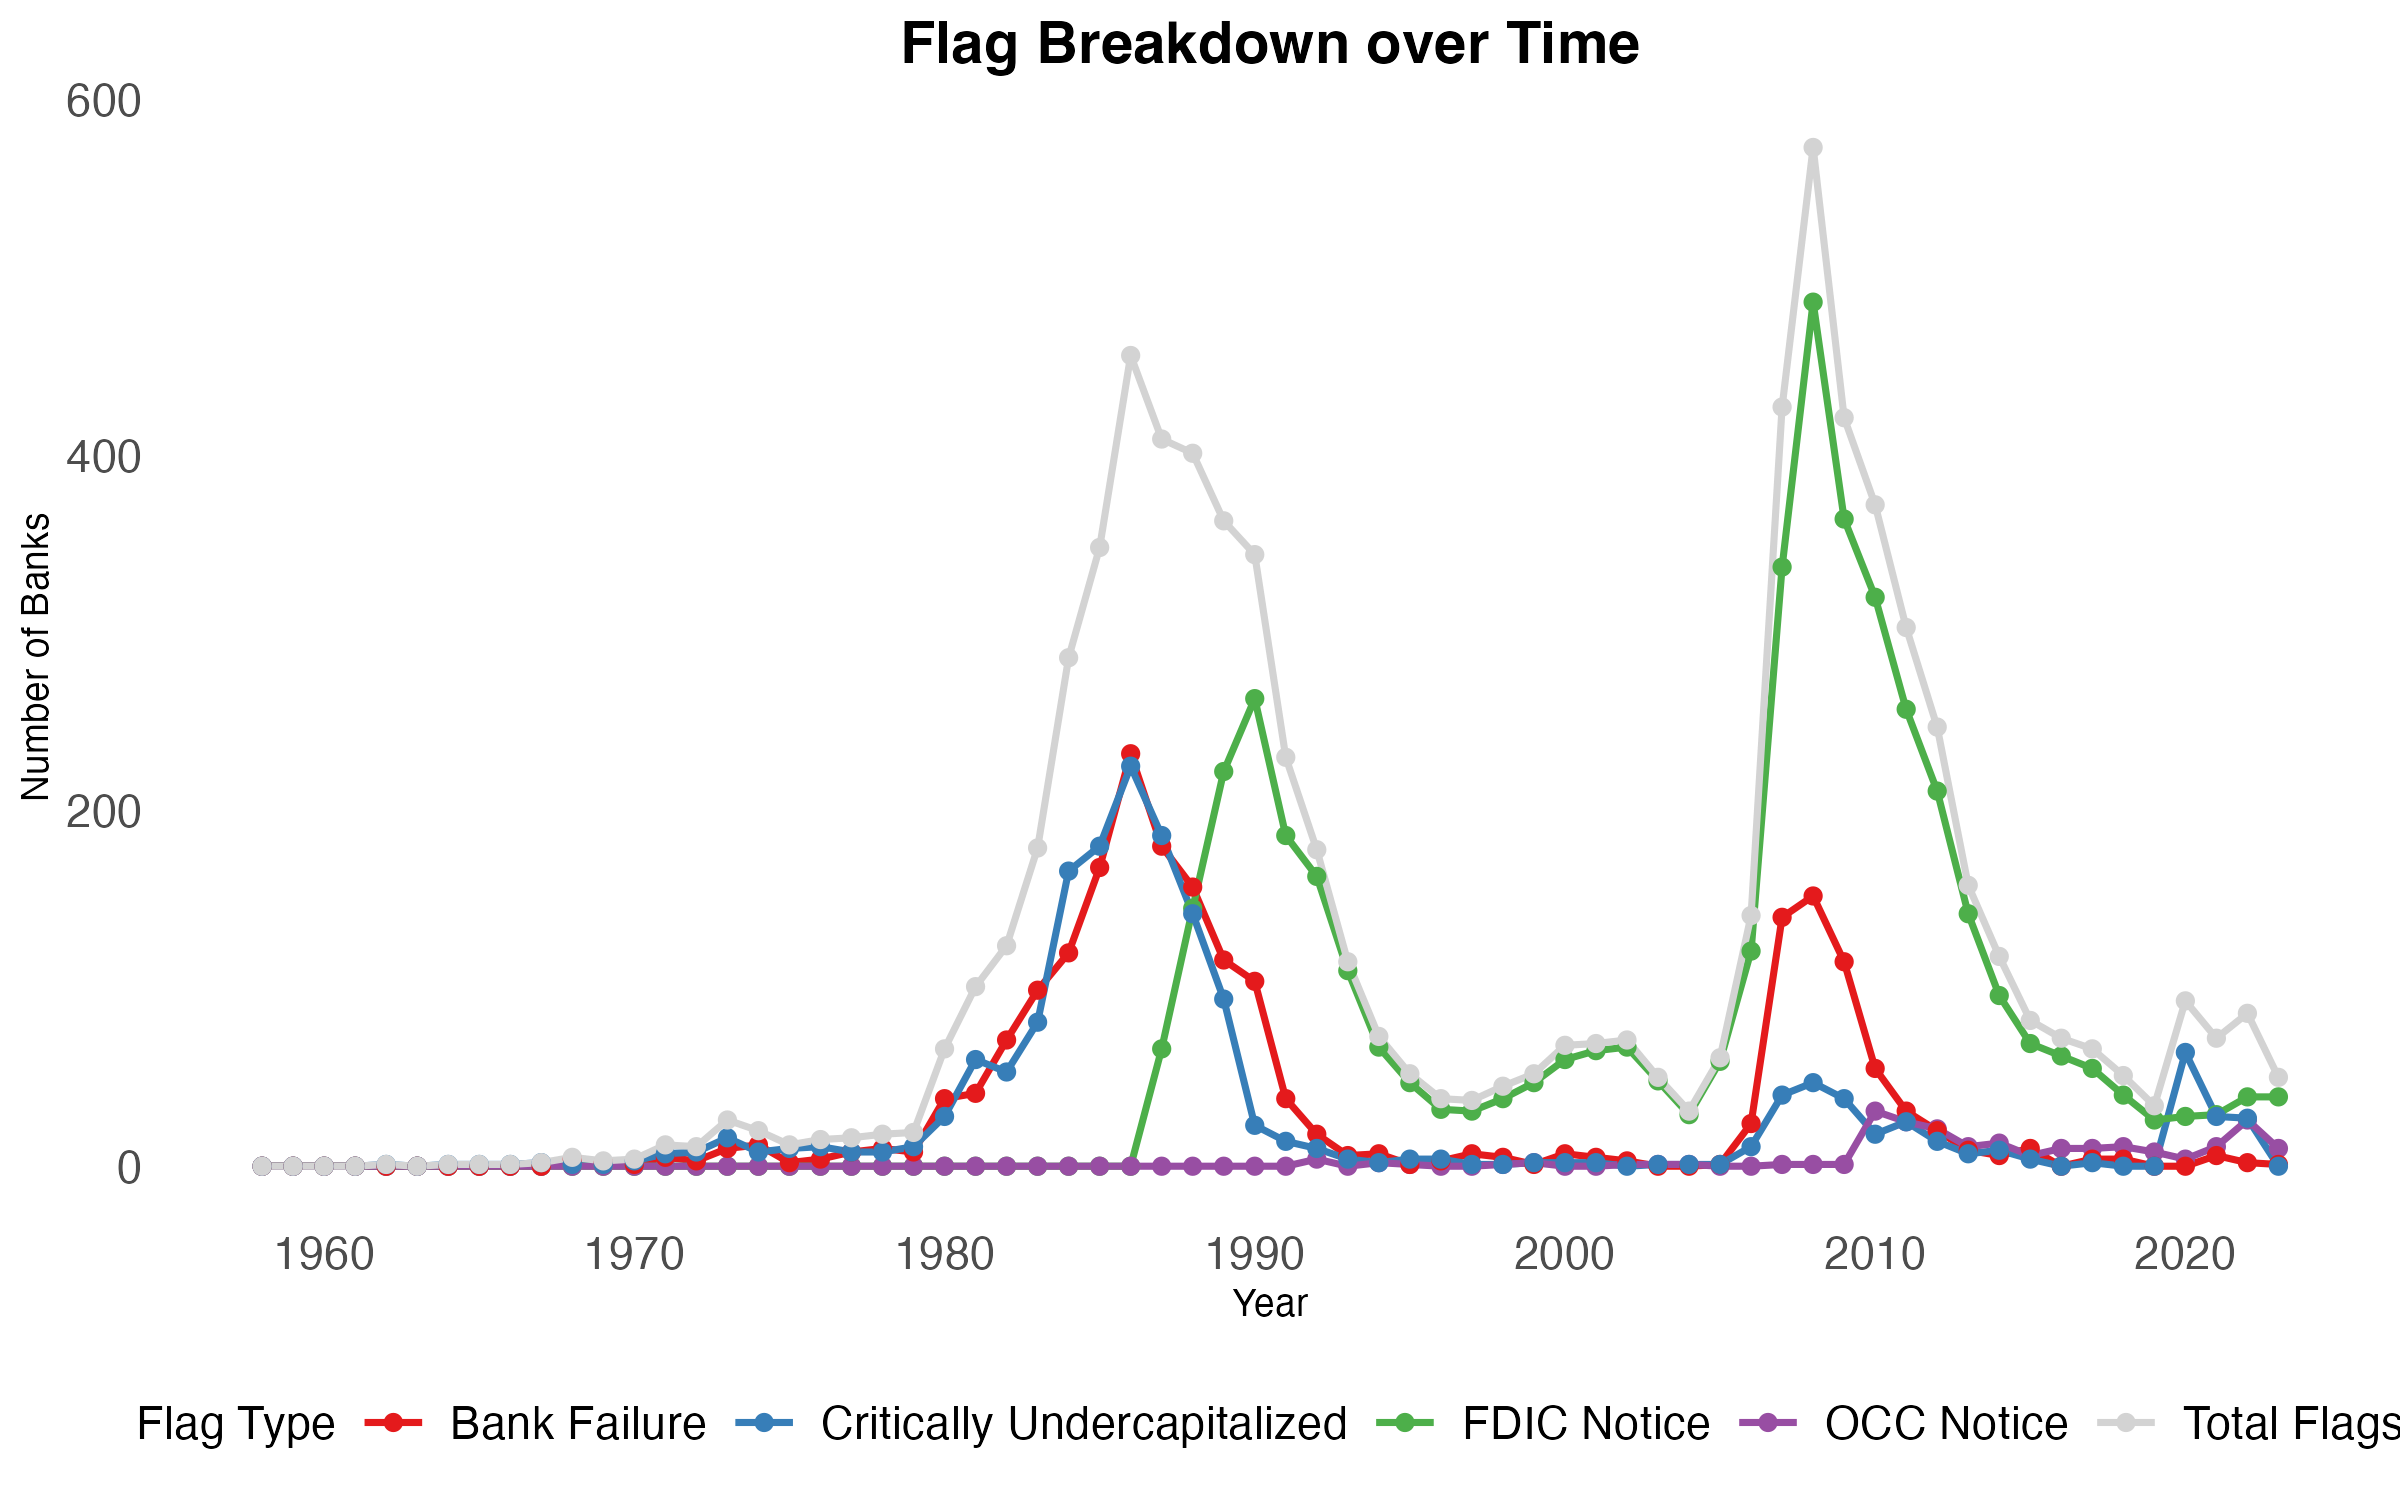
\includegraphics[width=0.75\linewidth]{flag_breakdown.png}
    \caption{Crisis Component Flags Over Time}
    \label{fig:flag-breakdown}
    
    
\end{figure}

Cohen's d, the standardized mean difference between the two classes, was therefore used as the primary measure, as it captures the magnitude of separation rather than merely its statistical detectability. The conventional benchmarks apply:  $|d| < 0.2$ indicates negligible separation, 0.2–0.5 small, 0.5–0.8 medium, and above 0.8 large. The distribution density charts were also analyzed for visibility of distribution differences of two labels across all featured. The plot backgrounds of features with Cohen's $|d| > 0.2$ were colored a light ivory color to emphasize the significant difference.

The results revealed a clear hierarchy across feature groups. Raw balance-sheet levels showed negligible effect sizes. Figure \ref{fig:04_eda-den-balance-1} shows the distribution differences of balance sheet components (logged values) in banks with no crisis detected next year and banks facing crisis next year. The overlap between the two distributions is nearly complete across all features, indicating that the absolute size of the balance sheet alone carries minimal discriminative power. The only feature that shows meaningful distributional separation is Other Real Estate Owned (OREO) which was acquired by the bank through foreclosure on defaulted loans. Higher OREO balances among pre-crisis banks indicate that asset quality problems have already begun to materialize, with borrowers unable to service their debt and the bank forced to seize the underlying collateral. Overall, the chart is consistent with the observation that bank failures occur across the entire size spectrum and confirms that balance-sheet levels serve primarily as denominators for the more informative ratio-based features.

\begin{figure}
    \centering
    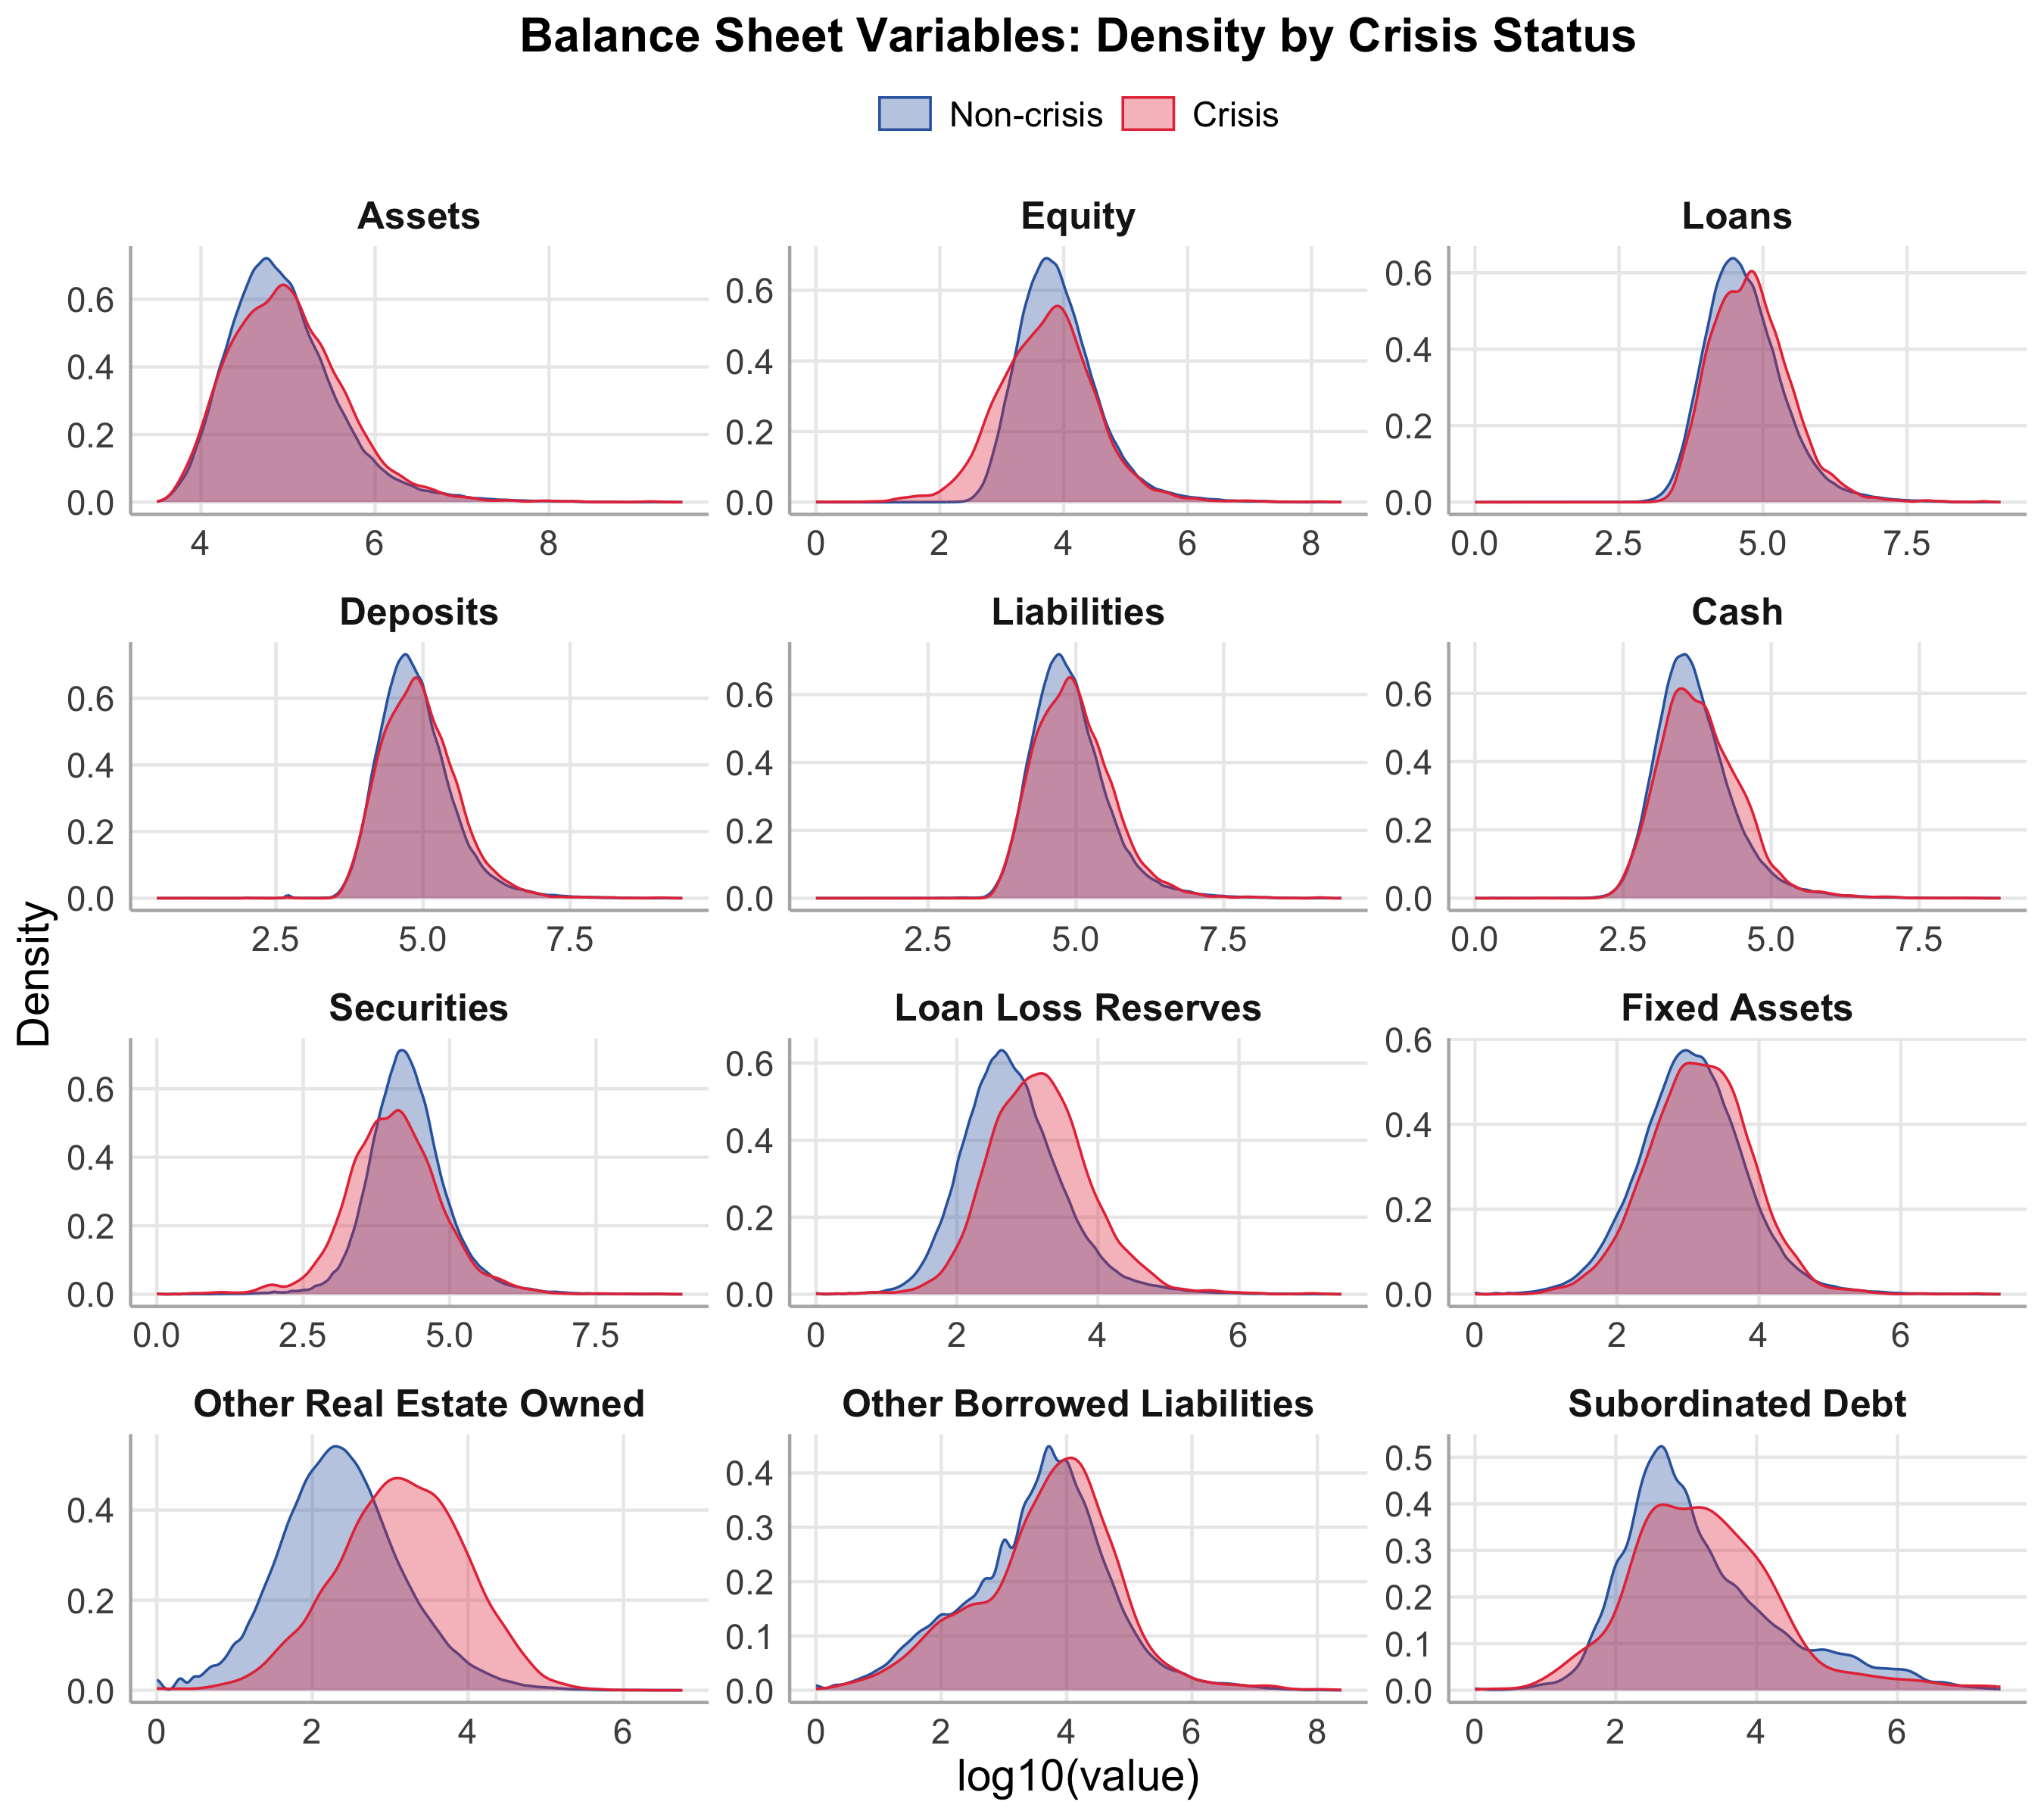
\includegraphics[width=0.75\linewidth]{04_eda-den-balance-1}
    \caption{Balance Sheet Components Distributions}
    \label{fig:04_eda-den-balance-1}
    
    
\end{figure}

Financial ratios, by contrast, exhibited the strongest separation. Figure \ref{fig:04_eda-den-ratios-1} shows that capital ratio, ROA, ROE, and NIM were all markedly lower among pre-crisis banks, with ROA and ROE frequently negative, indicating outright losses in the year before a crisis event. The non-performing loan ratio showed the opposite pattern, with substantially higher values among crisis banks, reflecting deteriorating asset quality. These findings confirm the CAMELS framework's emphasis on capital adequacy, earnings, and asset quality as the primary indicators of bank health.

\begin{figure}
    \centering
    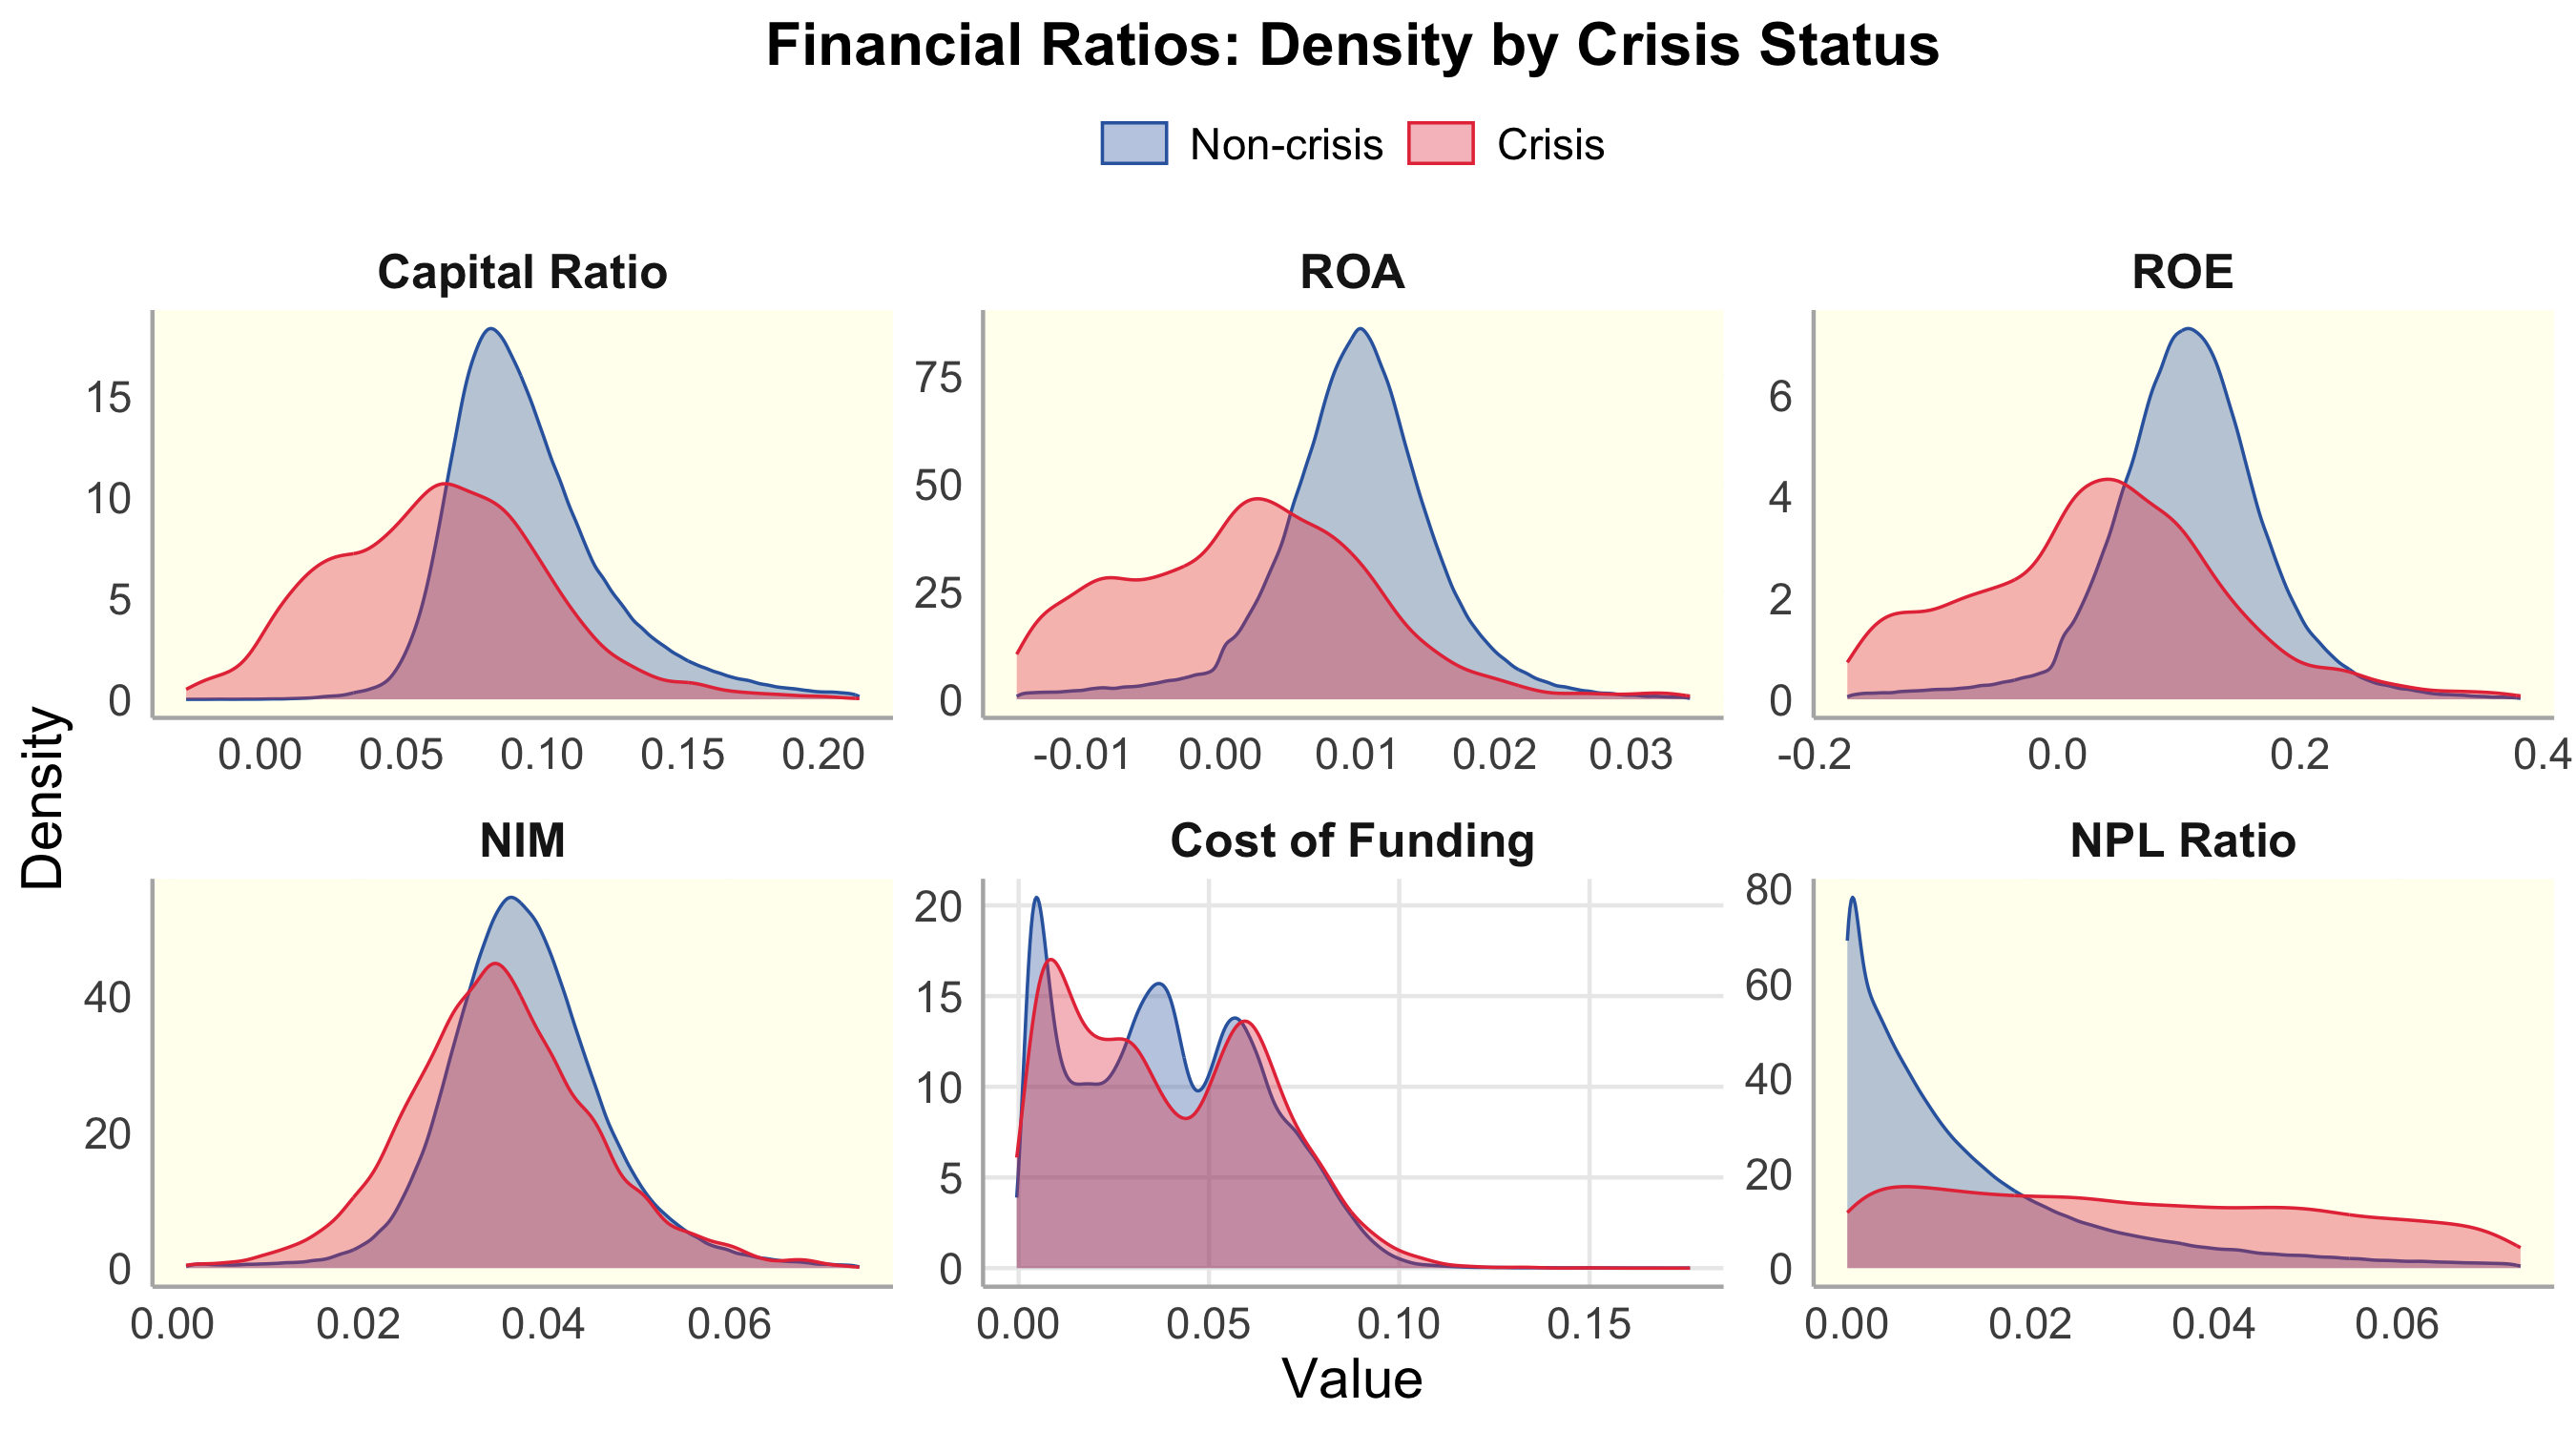
\includegraphics[width=0.75\linewidth]{04_eda-den-ratios-1}
    \caption{Financial Ratio Distributions}
    \label{fig:04_eda-den-ratios-1}
    
    
\end{figure}

Year-over-year dynamics provided additional discriminative signal. Banks approaching a crisis event typically exhibited negative growth rates across all major balance-sheet components as well as deteriorating financial ratios. Figure \ref{fig:04_eda-den-growth-ratio-1} shows that the distributions of balance-sheet growth rates for pre-crisis banks are shifted to the left relative to non-crisis banks, reflecting declining assets, deposits, loans, and equity in the year preceding a crisis event. The distributions of ratio changes exhibit a different pattern: rather than a clean shift, the crisis distributions are flatter and more dispersed, with heavier tails (especially left tails, indicating losses). This indicates that the direction of change, not just the level, carries predictive information, and supports the inclusion of both levels and first differences in the feature set.

Three-year rolling standard deviations revealed a particularly informative pattern. Earnings volatility, measured by the rolling standard deviation of ROA, was substantially elevated among pre-crisis banks, indicating persistent instability in the years preceding a crisis event. This finding is important because it suggests that medium-term instability is a hallmark of banks heading toward distress, and validates the construction of rolling-window features as complements to point-in-time ratios.


Intra-year quarterly dynamics showed moderate but meaningful separation. Maximum single-quarter declines in equity and deposits were larger among crisis banks, capturing acute stress events that annual snapshots mask. Within-year standard deviations of balance-sheet components were also elevated, consistent with heightened operational and financial volatility before distress.

\begin{figure}
    \centering
    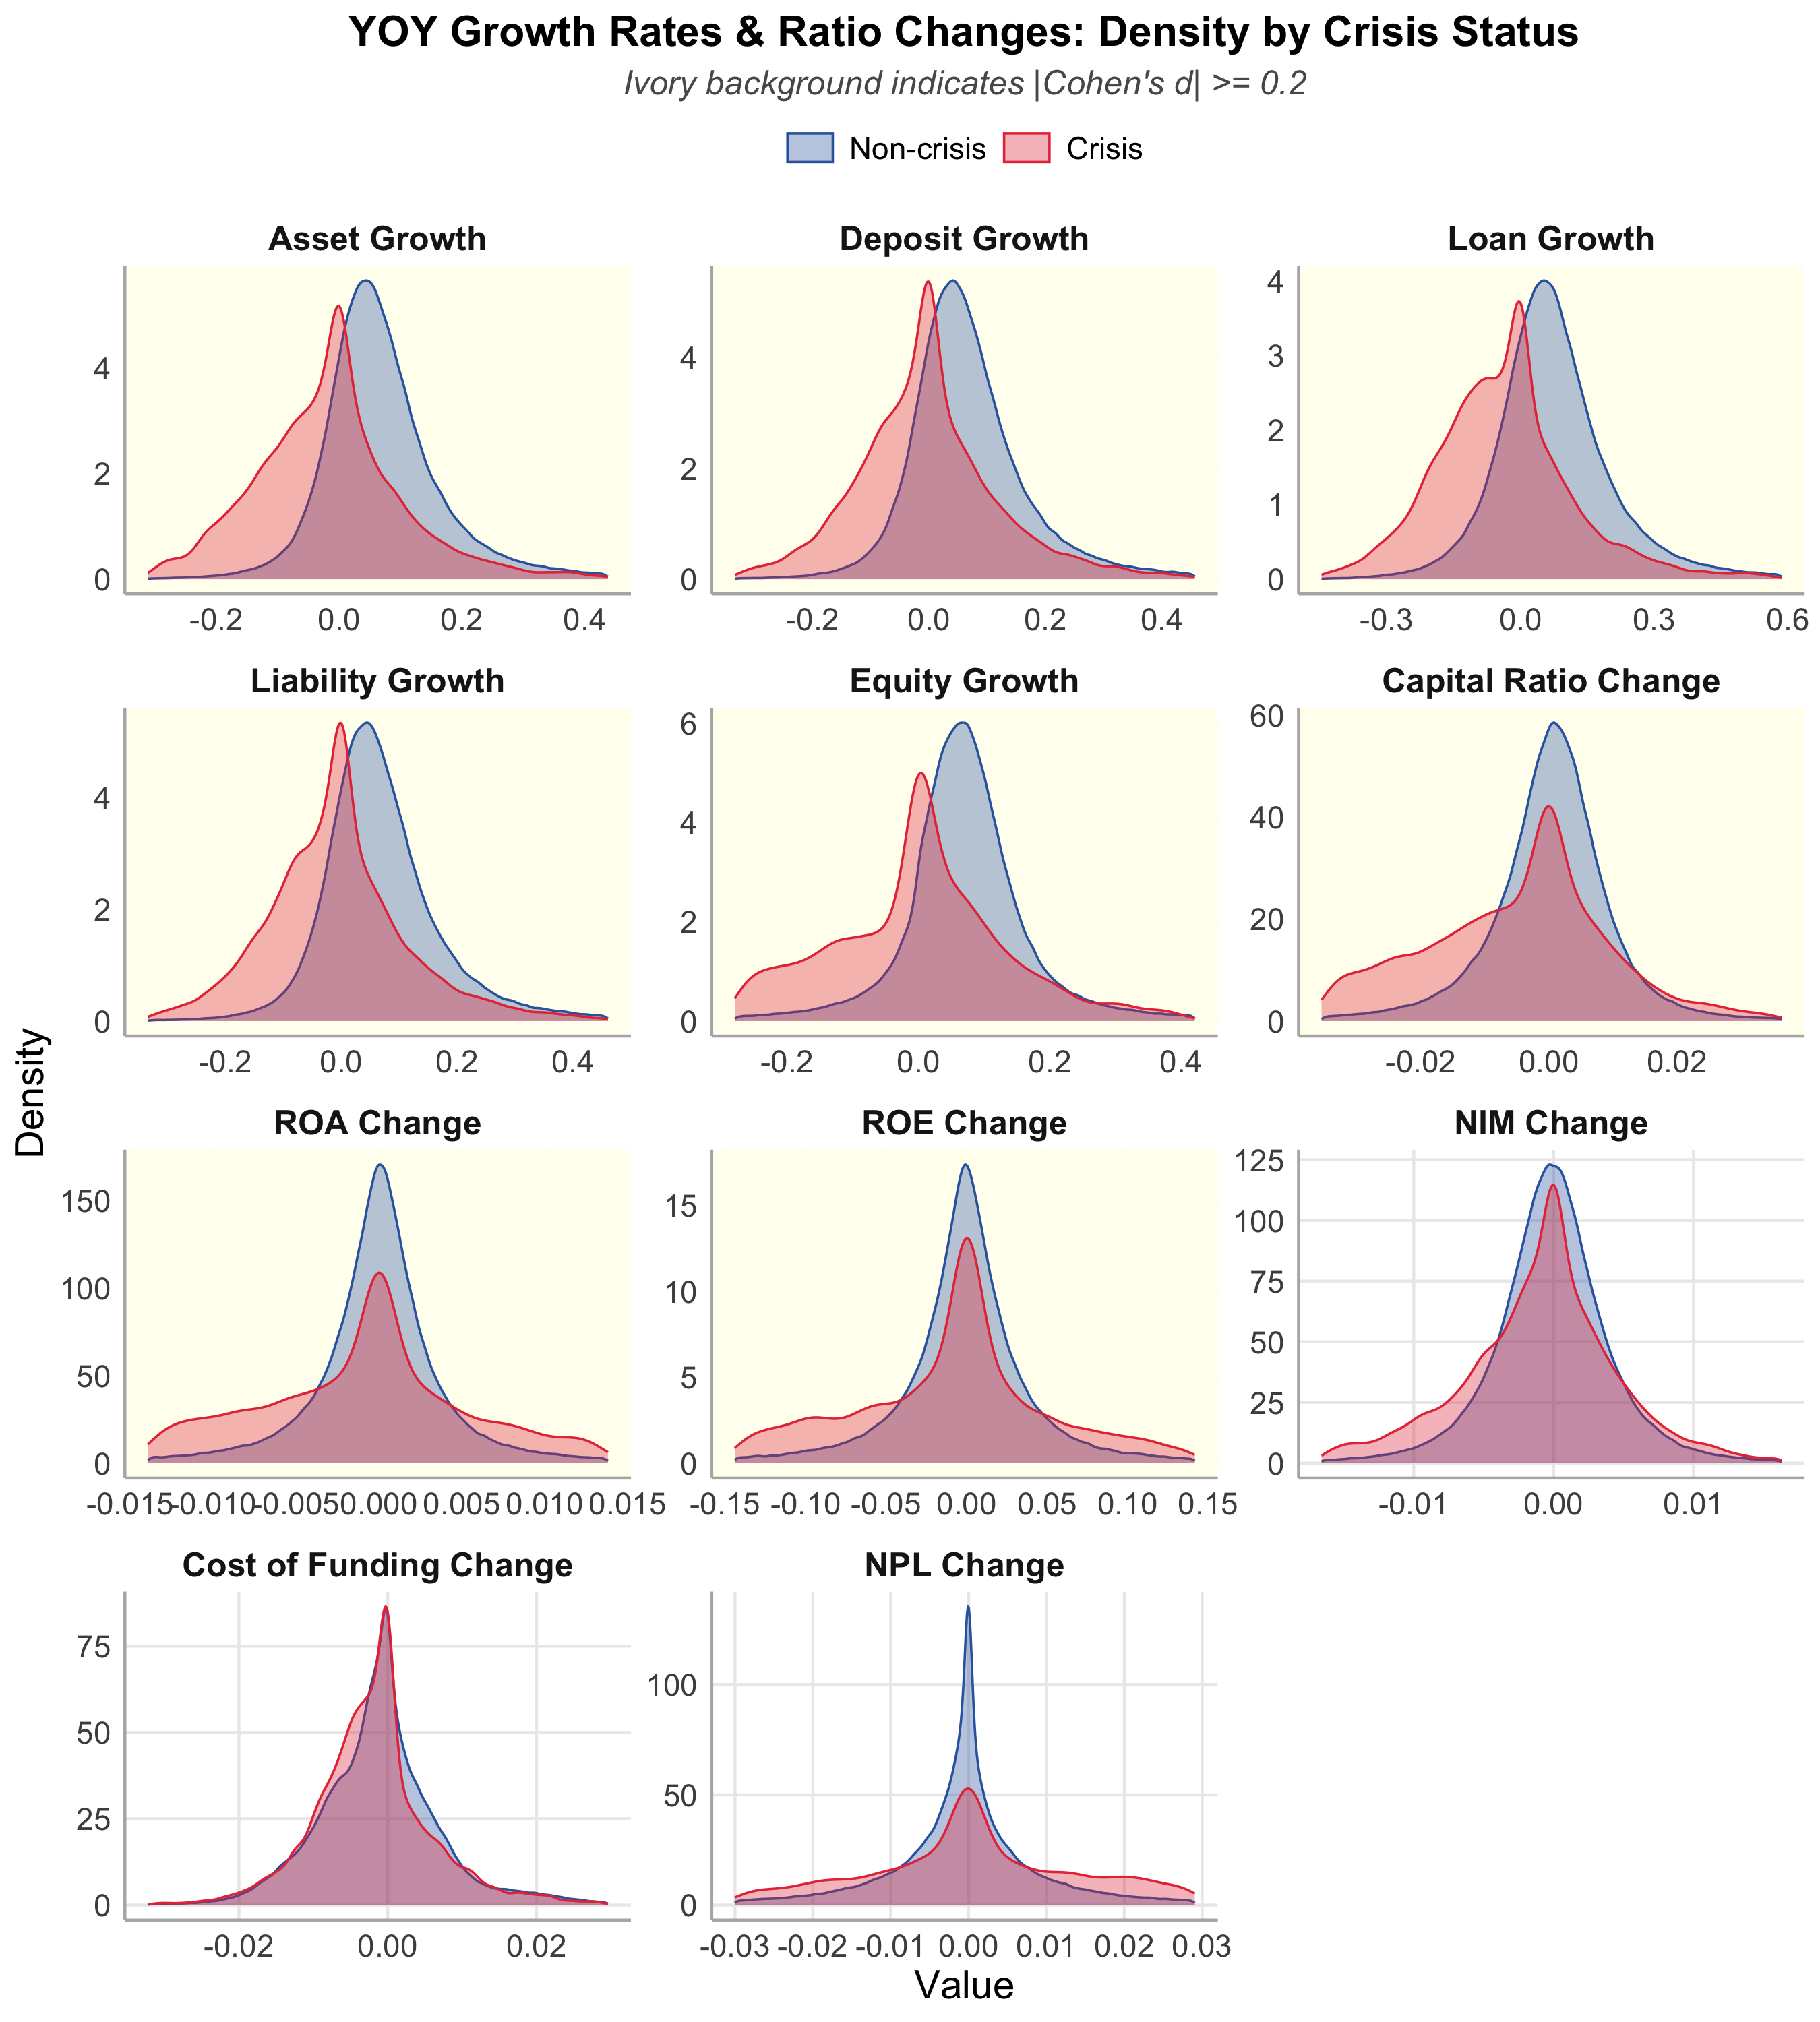
\includegraphics[width=0.75\linewidth]{04_eda-den-growth-ratio-1}
    \caption{Feature YOY Change Distributions}
    \label{fig:04_eda-den-growth-ratio-1}
    
    
\end{figure}

Loan composition features showed small but non-negligible effects. Banks with higher concentrations in commercial real estate and lower diversification across loan categories were somewhat more likely to experience crisis, consistent with the findings of Carmona et al. \cite{b8}. 

The features with meaningful discrimination are precisely those that the CAMELS framework and the bank failure literature identify as the core predictors of distress. Subsequently, features with negligible discrimination were removed from the feature selection stage to reduce noise and improve the interpretability of the model. 

Additionally, the features that were highly correlated with other features were also removed to eliminate the problem of multicollinearity within the features. The Variance Inflation Factor (VIF) Score was used for identifying the highly correlated features, and the features with a VIF Score greater than 10 were eliminated.

The final dataset used for training included 37 features and 380,447 rows of bank-year observations.


\subsection{Models Trained}
Three families of models were trained, progressing from simple pooled baselines through panel-aware econometric specifications to nonlinear tree ensembles. All models were trained on the same filtered feature set using the same temporal split, ensuring direct comparability.

\subsubsection{Baselines}
\textbf{Logistic regression} serves as the simplest benchmark. Features were median-imputed, winsorized at the 1st/99th percentiles, and standardized, with all statistics computed on the training window only. Class imbalance was addressed via inverse-frequency weighting. 

\textbf{LASSO (L1-regularized logistic regression)} extends the pooled logit by adding an L1 penalty that shrinks uninformative coefficients to exactly zero, performing embedded feature selection. The regularization strength was selected via temporal cross-validation maximizing PR-AUC. 

\subsubsection{Panel-Aware Linear Models}
\textbf{Mixed Effect Logit (Mundlak correlated random effects)} model was tested. For each time-varying feature, the bank-level mean across all observed years is added as an additional regressor. The coefficient on the original feature then captures within-bank variation, while the coefficient on the bank mean captures between-bank variation. This decomposition is equivalent to a correlated random effects model under standard assumptions \cite{b21}, \cite{b22} and provides interpretive value that no other model in the pipeline offers.

\textbf{Generalised Estimating Equations (GEE)} model was also used to address the model structure of the data \cite{b23}. Two correlation structures are fitted in parallel exchangeable (assumes a constant within-bank correlation and acts as the random-effects assumption) and independence (ignores within-bank correlation and is equivalent to pooled logit with robust standard errors). GEE coefficients are consistent even if the working correlation is wrong (the theoretical attraction). Unlike GLMM it doesn't estimate per-bank random intercepts, so it scales. Unlike fixed-effects logit, it can predict on unseen banks.

\subsubsection{Tree-based Models}
\textbf{XGBoost.} A gradient-boosted decision tree ensemble that sequentially adds weak learners, each correcting the residual errors of the previous ones. Hyperparameters were tuned via Optuna (100 trials) using the temporal cross-validation folds, with PR-AUC as the objective. Early stopping within each fold determined the number of boosting rounds. 

\textbf{LightGBM.} A leaf-wise gradient boosting implementation that grows trees by splitting the leaf with the highest gain, rather than level-wise as in XGBoost. This typically produces deeper, more expressive trees for the same number of leaves. Tuned with the same Optuna framework and temporal CV, using LightGBM-idiomatic parameters. 

\textbf{Random Forest.} An ensemble of independently trained decision trees, each fit on a bootstrap sample of the training data with a random subset of features considered at each split. Unlike boosting, trees are trained in parallel and their predictions are averaged — reducing variance rather than bias. Included because it represents a fundamentally different ensemble strategy and is the most commonly reported ML model in the bank failure literature \cite{b1}, \cite{b4}. 

\subsection{Evaluation Framework}
\textbf{Primary metric: PR-AUC.} Precision-recall area under the curve was chosen as the primary evaluation metric because the crisis label is severely imbalanced. ROC-AUC can appear deceptively high on imbalanced data — a model that rarely predicts the positive class achieves high specificity almost for free, inflating the ROC curve \cite{b1}. PR-AUC focuses exclusively on the positive class and penalizes models that achieve high recall only by flooding predictions with false positives. The no-skill baseline for PR-AUC equals the positive rate, providing a natural reference point.

\textbf{Threshold selection: F2 score on validation.} The conventional default of 0.5 is inappropriate at low positive rates. Instead, the threshold maximizing the F2 score was selected on the validation set. F2 weights recall twice as heavily as precision, reflecting the asymmetric cost structure in bank supervision: a missed crisis (Type II error) carries far greater consequences than a false alarm (Type I error), which results only in additional supervisory attention to a healthy bank.

\subsection{Interpretability}
\textbf{Linear model coefficients}. For the Pooled logit, LASSO, Mixed Effects, and GEE models, the estimated coefficients are directly interpretable as the change in log-odds of crisis per one-standard-deviation increase in the feature (since all features are standardized prior to fitting). Coefficients from the LASSO model additionally indicate which features the regularization retained versus shrunk to zero, serving as an embedded feature selection mechanism. The Mixed Effects specification decomposes each coefficient into a within-bank effect (how a bank's deviation from its own historical average relates to crisis risk) and a between-bank effect (how a bank's long-run average level relates to crisis risk), providing insight unavailable from any other model in the pipeline.

\textbf{SHAP (SHapley Additive exPlanations)}. For the tree-based ensembles (XGBoost, LightGBM, Random Forest), TreeSHAP \cite{b11} was applied to decompose each individual prediction into per-feature contributions. For a given bank-year, the SHAP value of a feature indicates how much that feature's value pushed the predicted crisis probability above or below the population average. Aggregating absolute SHAP values across the test set produces a global feature importance ranking grounded in cooperative game theory, which is more stable and theoretically principled than gain-based or permutation-based importance measures. 

\subsection{Symmetry Test}
The central analytical contribution of this project compares SHAP-based driver structures across the crisis and growth models. 

To test the symmetry between growth and crisis, another label, indicating growth was constructed. The label assigned positive class to the banks in year t if in year t+1 the bank's net income grew by 30\% or the ROE grew by 5 percentage points. This requirement is set to ensure that flagged banks are experiencing genuine financial strengthening rather than mechanical percentage swings from a near-zero base.The same models were trained to predict growth and the SHAP values for tree-based models were computed. For the symmetry test the SHAP values of the LightGBM model were used since it was the best performer among the models.

For each feature appearing in the top 10 by mean $|\mathrm{SHAP}|$ for either label, the test proceeds as follows: (1) bin all test-set observations into 20 quantile groups by feature value, (2) compute the mean SHAP value within each bin separately for the crisis and growth models, (3) compare the crisis SHAP curve against the growth SHAP curve using Spearman rank correlation. 

\subsection{Tools and Software}
Data exploration, cleaning, and feature engineering were implemented in R (v4.3) using the tidyverse ecosystem, with the effsize and car packages for Cohen's d computation and VIF analysis respectively. All modeling, evaluation, and interpretability analyses were implemented in Python (v3.11). Tree-based models were trained using XGBoost (v2.0), LightGBM (v4.0), and scikit-learn (v1.3) for Random Forest. Hyperparameter optimization was performed with Optuna (v3.4) using SQLite-backed storage for resumable studies. Panel-aware linear models used statsmodels (v0.14) for GEE. SHAP values were computed using the shap library (v0.44). All figures were produced with ggplot, matplotlib and seaborn. 

\section{Results}
\subsection{Crisis Prediction Model Performance}

Table \ref{tab:test_metrics_crisis} presents the test-set performance of all models on the crisis label. 

\begin{table}
\caption{Test-set performance: Crisis target.}
\label{tab:test_metrics_crisis}
\begin{tabular}{lrrrrr}
\toprule
model & accuracy & recall & precision & pr\_auc & roc\_auc \\
\midrule
Logit & 0.778 & 0.604 & 0.037 & 0.074 & 0.737 \\
Lasso & 0.123 & 0.919 & 0.014 & 0.038 & 0.656 \\
Mixed Effects Logit & 0.271 & \textbf{0.907} & 0.017 & 0.070 & 0.745 \\
GEE & 0.406 & 0.818 & 0.019 & 0.156 & 0.723 \\
XGBoost & 0.781 & 0.689 & 0.043 & \textbf{0.216} & 0.797 \\
LightGBM & 0.880 & 0.573 & 0.065 & 0.202 & 0.794 \\
Random Forest & \textbf{0.934} & 0.513 & \textbf{0.108} & 0.196 & \textbf{0.820} \\
\bottomrule
\end{tabular}
\end{table}

The results reveal that tree-based models dominate. XGBoost achieves the highest PR-AUC (the primary metric), followed closely by LightGBM and Random Forest. The no-skill baseline PR-AUC at the 1.99\% positive rate is 0.020. The narrow spread among the three tree models suggests that the predictive signal in the data is well captured by any competent tree ensemble, and the choice among them is secondary to the choice between tree and linear approaches. ROC-AUC values of 0.79–0.82 confirm strong discriminative ability, though this metric is less informative at the 1.99\% positive rate.

\subsection{Cross-Model Feature Importance}
To compare feature importance across model families, a consensus heatmap (Figure \ref{fig:feature-heatmap}) was constructed by normalizing each model's feature importance values to [0, 1] (absolute standardized coefficients for linear models, mean $|\mathrm{SHAP}|$ for tree models) and displaying the top 20 features across all six specifications. Value 1.0 indicates that the feature was the most important while 0.0 indicates the least important feature out of the selected features.

\begin{figure}
    \centering
    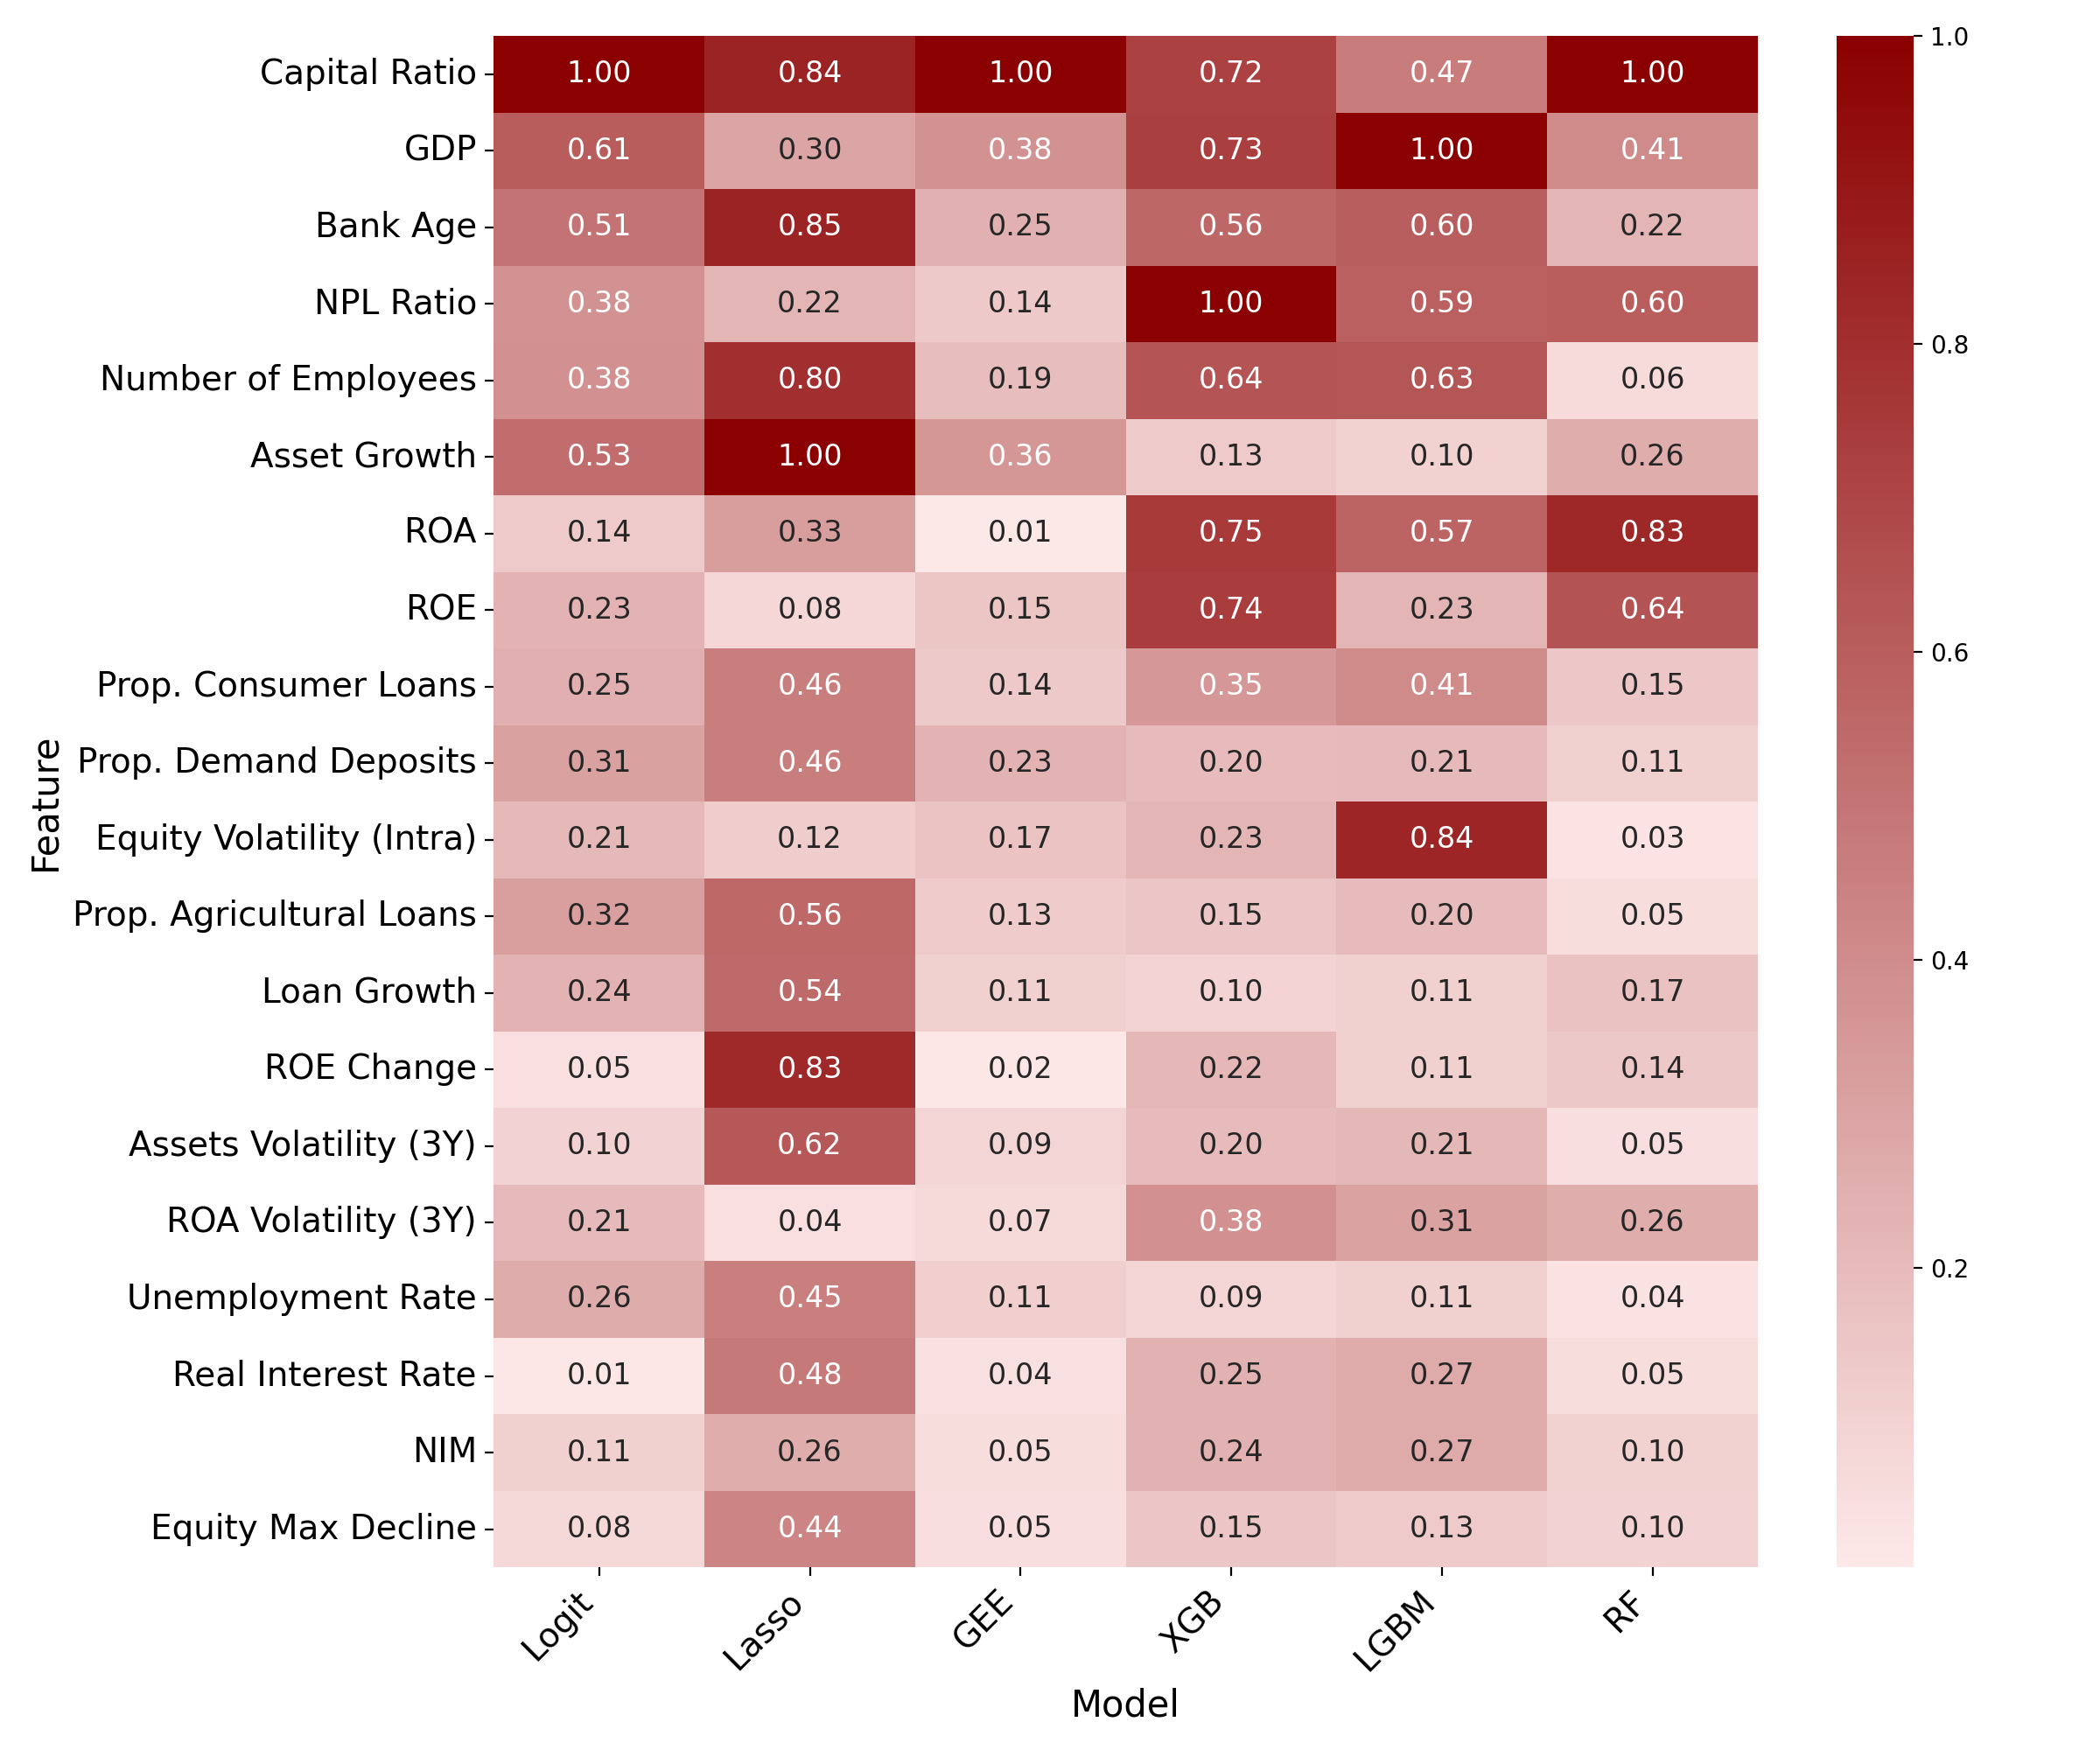
\includegraphics[width=1\linewidth]{consensus_importance_crisis}
    \caption{Normalized Feature Importance Consensus Heatmap}
    \label{fig:feature-heatmap}
    
    
\end{figure}

\section{Analysis and Validation}
The dominant finding that model performance results suggest is that nonlinear feature interactions, captured by tree ensembles, carry substantially more predictive information than either pooled or panel-aware linear specifications. The practical implication is that a regulator using XGBoost would identify crisis banks 11 times more effectively than random screening.

The relatively low absolute PR-AUC values reflect the difficulty of the prediction task at a 1.99\% positive rate, not a model failure. Given the imbalance, even a well-calibrated model must trade precision for recall: at the F2-optimal threshold, the best models catch roughly half of true crises while keeping false alarm rates below 2\%. 

According to Figure \ref{fig:feature-heatmap}, capital ratio is the most universally important feature, ranking first for Logit, GEE, and Random Forest, and in the top tier for all other models. This broad consensus confirms the CAMELS framework's emphasis on capital adequacy as the primary early warning signal.

NPL ratio and ROA reveal the sharpest disagreements between linear and tree models. NPL ratio is the single most important feature for XGBoost and ranks highly for LightGBM and Random Forest, yet receives low importance from GEE and Lasso. ROA follows the same pattern: it's dominant for Random Forest and XGBoost but nearly irrelevant for GEE. These divergences reflect nonlinear threshold effects: asset quality deterioration and profitability losses may only become predictive beyond certain levels that tree splits capture naturally but linear models cannot represent without explicit interaction terms.

Bank age and number of employees (size) are prominent across multiple specifications. Both rank highly for Lasso and maintain moderate importance across the tree models, confirming that institutional maturity and operational scale carry genuine predictive signal beyond what financial ratios alone provide.

Growth rates exhibit the opposite pattern. Asset growth is the single most important feature for Lasso but receives consistently low importance from all three tree ensembles. Linear models lean on balance-sheet trajectories, which have a roughly monotonic relationship with crisis risk, while trees access equivalent signal through more complex feature interactions.

GDP is the most important feature for LightGBM, suggesting that tree models exploit macroeconomic context through interactions with bank-level characteristics rather than as a direct additive effect. LightGBM also assigns unusually high importance to intra-year equity volatility — a feature that other models largely ignore, indicating that this model captures short-term stress dynamics that other specifications miss.

Lasso exhibits a distinctive importance profile, assigning high weight to ROE change and three-year asset volatility alongside the growth rates, reflecting its tendency to select a sparse set of high-signal features through regularization. By contrast, the tree models distribute importance more broadly across profitability, asset quality, and composition features.

The features where linear and tree models diverge most are precisely those where nonlinear effects are economically expected, providing a structural explanation for the predictive gap documented in Table \ref{tab:test_metrics_crisis}.

\subsection{Symmetry Analysis}

\begin{figure}
    \centering
    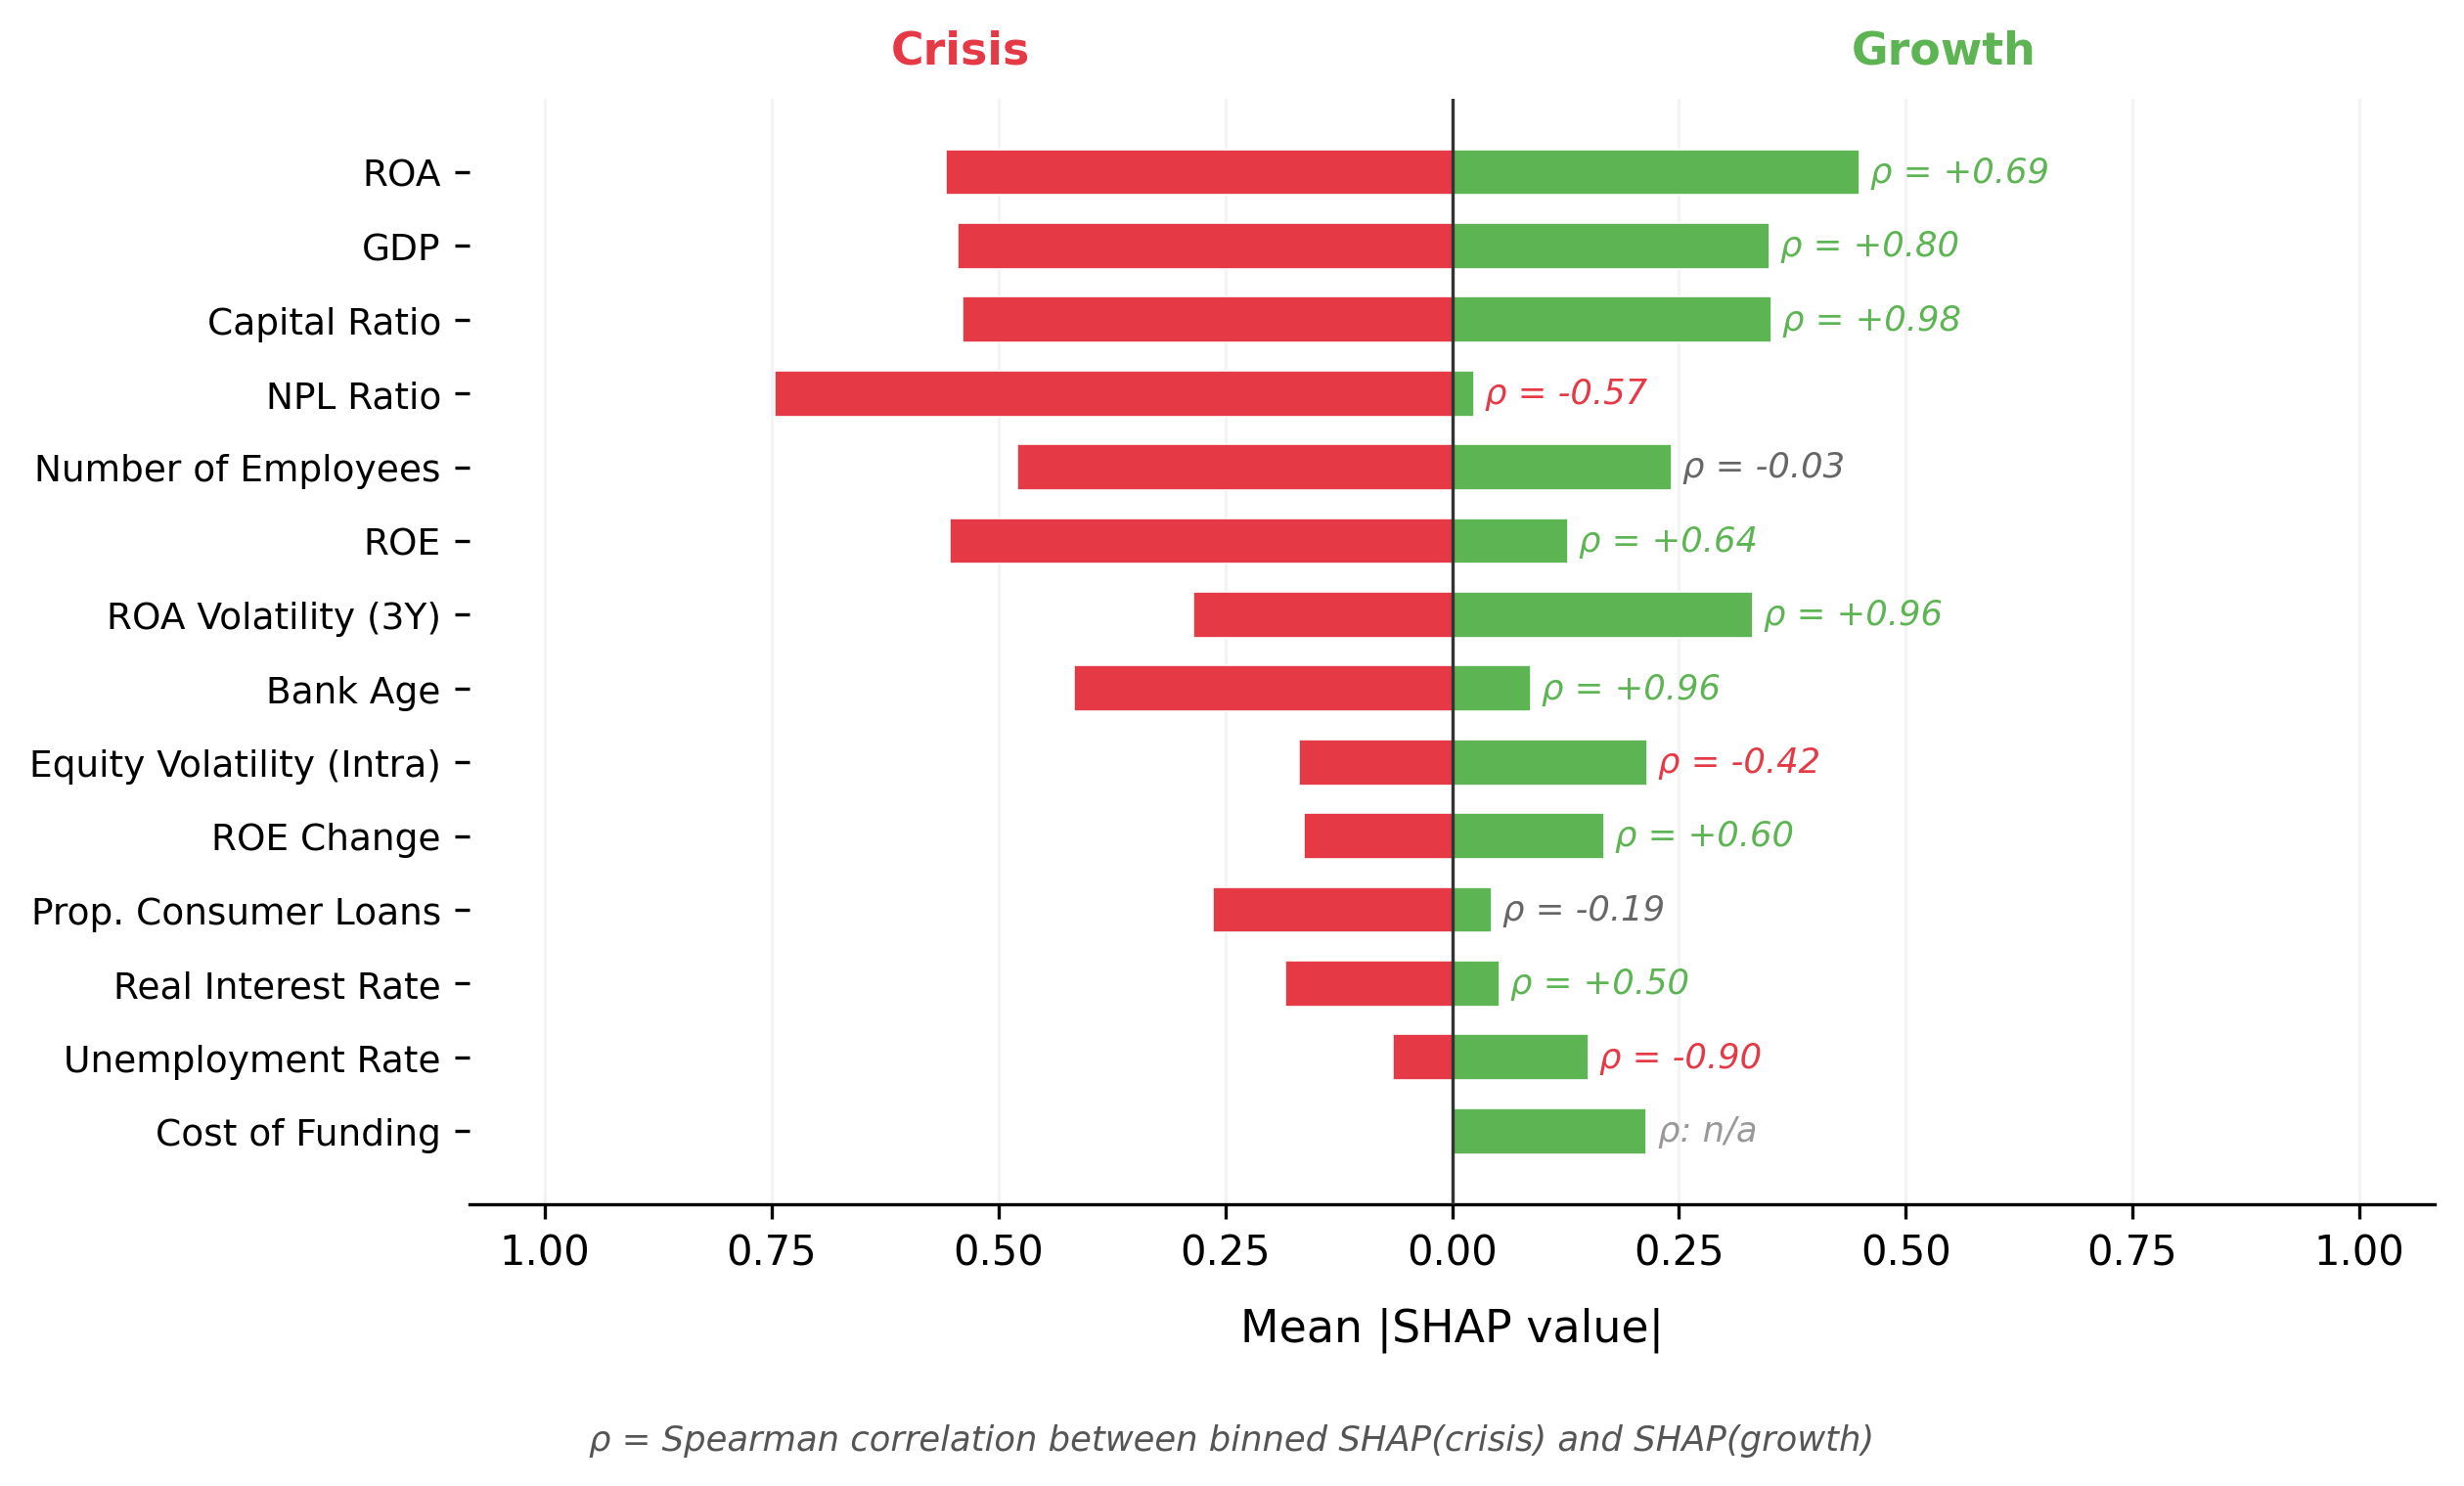
\includegraphics[width=1\linewidth]{xgb_shap_symmetry_mirror}
    \caption{Top 10 Features by Importance for Crisis and Growth}
    \label{fig:xgb_shap_symmetry_mirror}
    
    
\end{figure}

Figure \ref{fig:xgb_shap_symmetry_mirror} shows the results of the symmetry test. The chart reveals insightful information regarding the drivers of crisis and growth. 

Several of the most important features exhibit strong positive correlations, meaning the same feature values that push a bank toward crisis also push it toward growth. Capital ratio, ROA volatility, bank age, GDP, ROA, and ROE all show high positive correlation. This is a counterintuitive but economically coherent finding: undercapitalized banks with volatile earnings are simultaneously at the highest risk of failure and the most likely to experience sharp income recovery, while well-capitalized stable banks are safe from crisis but unlikely to see dramatic financial improvement. Crisis and growth are not opposites on a single axis rather they are both characteristics of volatile, high-risk institutions, with the stable middle experiencing neither.

A second group of features acts as genuine mirrors between the two outcomes. NPL ratio, unemployment rate, and intra-year equity volatility show negative correlations, meaning they drive crisis and growth in opposite directions. High non-performing loans and elevated unemployment push toward crisis and away from growth, while the reverse conditions favor growth and reduce crisis risk. These are the features where the intuitive opposite relationship holds. They represent structural damage to asset quality and the macroeconomic environment that unambiguously harms bank prospects. Negative correlation coefficient for intra-year equity volatility indicates that within year high volatility is harmful: it drives crisis and does not allow growth. At the same time three-year volatility is driving both crisis and growth.

A third group of features matters primarily for one outcome. Cost of funding is important for the growth model but carries minimal weight for crisis. Conversely, NPL ratio is among the most important crisis features but contributes relatively little to growth predictions. Number of employees is moderately important on both sides but with near-zero correlation, meaning bank size matters for both outcomes but through entirely unrelated mechanisms.


\subsection{Limitations}
While the proposed framework yields strong predictive performance and high-resolution interpretability, several limitations should be acknowledged. First, the models were trained exclusively on US banking data; therefore, the specific feature interactions may not generalize perfectly to international banking systems with different regulatory environments. Second, the "crisis" target relies on historical failure events and regulatory interventions, which can sometimes be imperfect or lagging indicators of underlying distress. It would be effective to include Tier 1 Capital Adequacy Ratio and Total Capital Adequacy Ratio in the crisis label but due to non-availability of Tier 1 Capital level and Risk Waited Assets in the datasets and or in any other publicly available source, it was not possible to implement. Third, the extreme class imbalance and low positive rate inherently constrains the theoretical ceiling for model precision. Lastly, the threshold used to define the "growth" label is somewhat arbitrary, and alternative definitions for growth could shift the specific rank-order of feature importance on the positive side of the spectrum.

\subsection{Summary of Findings}
Overall, the project successfully achieved its primary objectives. The proposed framework produced an effective, interpretable early-warning model for bank distress. The performance metrics clearly demonstrate that non-linear machine learning models substantially outperform traditional linear approaches when navigating the complex, high-dimensional nature of banking data. According to the best performing model, XGBoost, the main drivers of crisis are NPL Ratio, Capital Ratio and GDP. Furthermore, the SHAP symmetry analysis revealed insightful findings about same features being responsible for crisis and growth indicating that high-risks and volatility can be followed by both crisis and growth, and stakeholders should take into account both outcomes when taking risks. 

\section{Discussion and Conclusion}
The results show that tree-based machine learning models substantially outperform traditional linear approaches. XGBoost achieved the strongest overall performance, followed closely by LightGBM and Random Forest, indicating that bank distress is driven by nonlinear relationships and feature interactions that linear models cannot fully capture. Capital adequacy, profitability, earnings stability, and asset quality emerged as the most important predictors across models, confirming the central findings of the CAMELS-based banking literature.

The feature importance rankings align with Petropoulos et al. \cite{b4} and the broader CAMELS literature: capital adequacy, profitability, and asset quality dominate across all model families, confirming that these indicators remain the most reliable predictors of bank distress even on a substantially longer panel.

The underperformance of panel-aware linear models relative to pooled logit is notable but not unprecedented. The Mundlak specification doubles the feature count by adding bank-level means, which likely introduces overfitting on the training window that does not transfer to the structurally different test period (post-COVID, rising interest rates). GEE performs best among the linear family, suggesting that the within-bank correlation structure adds computational cost without predictive benefit in a forecasting context where unseen banks receive zero random effects.

The main analytical contribution of the project is the SHAP symmetry framework comparing the drivers of crisis and growth outcomes. The analysis yields perhaps the most unexpected finding of this study. It is mostly believed that the same indicators separate both groups in opposite directions. The results suggest a more nuanced picture: crisis and growth are not opposites but rather co-products of financial volatility. Banks with low capital, unstable earnings, and high sensitivity to macroeconomic conditions occupy a high-variance regime where both dramatic failure and dramatic recovery are possible, while well-capitalized, stable institutions inhabit a low-variance regime where neither outcome is likely. 

The symmetry finding carries direct implications for supervisory practice. A regulator relying on a single crisis-score would inadvertently assign high risk to banks that are simultaneously the most likely to recover, since the same volatility that produces failure risk also produces recovery potential. Separating crisis and growth models allows examiners to distinguish genuinely deteriorating institutions from volatile-but-viable ones — a distinction that a unidimensional risk score cannot make.

The project has several practical implications. The results demonstrate that interpretable machine learning models can improve early-warning systems for bank supervision while also providing economically meaningful insights into the structure of bank health. 

Future work could extend the framework to international banking systems, alternative definitions of growth and distress, and more advanced architectures such as sequence or graph-based models. Incorporating market-based variables may also further improve predictive performance. The models can be trained with data from different countries to make them universally applicable.

Overall, the project successfully achieved its objectives. It developed a robust and interpretable framework for bank distress prediction and introduced a novel symmetry-based analysis showing that the determinants of banking crisis and banking growth are only partially overlapping.

\begin{thebibliography}{00}
\bibitem{b1} A. Citterio, "Bank failure prediction models: Review and outlook," Socio-Economic Planning Sciences, vol. 92, art. no. 101818, Apr. 2024, doi: 10.1016/j.seps.2024.101818.

\bibitem{b2} F. Betz, S. Oprică, T. A. Peltonen, and P. Sarlin, "Predicting distress in European banks," Journal of Banking \& Finance, vol. 45, pp. 225–241, Aug. 2014, doi: 10.1016/j.jbankfin.2013.11.041.

\bibitem{b3} D. Malikkidou and W. Strohbach, "Predicting bank distress in Europe: Using machine learning and a novel definition of distress," European Banking Authority, Paris, France, EBA Staff Paper Series No. 21, Jan. 2025.

\bibitem{b4} A. Petropoulos, V. Siakoulis, E. Stavroulakis, and N. E. Vlachogiannakis, "Predicting bank insolvencies using machine learning techniques," International Journal of Forecasting, vol. 36, no. 3, pp. 1092–1113, Jul. 2020

\bibitem{b5} A. Cerqua, M. Letta, and G. Pinto, "On the (Mis)Use of machine learning with panel data," Oxford Bulletin of Economics and Statistics, early view, 2025, doi: 10.1111/obes.70019.

\bibitem{b6} W. H. Beaver, "Financial ratios as predictors of failure," Journal of Accounting Research, vol. 4, pp. 71–111, 1966.

\bibitem{b7} E. I. Altman, "Financial ratios, discriminant analysis and the prediction of corporate bankruptcy," Journal of Finance, vol. 23, no. 4, pp. 589–609, 1968.

\bibitem{b8} P. Carmona, F. Climent, and A. Momparler, "Predicting failure in the U.S. banking sector: An extreme gradient boosting approach," Int. Rev. Econ. \& Finance, vol. 61, pp. 304–323, 2019.

\bibitem{b9} H. H. Le, "Predicting bank distress using XGBoost and SHAP-based interpretation," Doctoral thesis, 2023.

\bibitem{b10} A. Ekinci and S. Sen, "Forecasting bank failure in the U.S.: A cost-sensitive approach," Comput. Econ., vol. 63, pp. 1–25, 2024.

\bibitem{b11} S. M. Lundberg and S.-I. Lee, "A unified approach to interpreting model predictions," in NeurIPS, vol. 30, 2017, pp. 4765–4774.

\bibitem{b12} R. A. Cole and L. J. White, "Déjà vu all over again: The causes of U.S. commercial bank failures this time around," J. Fin. Serv. Res., vol. 42, no. 1–2, pp. 5–29, 2012.

\bibitem{b13} A. Babii, R. T. Ball, E. Ghysels, and J. Striaukas, "Machine learning panel data regressions with heavy-tailed dependent data," J. Econometrics, vol. 237, art. 105315, 2023.

\bibitem{b14} Correia, Sergio A., Stephan Luck, and Emil Verner. “Failing Banks,” The Quarterly Journal of Economics, Volume 141, Issue 1, February 2026, Pages 147–204

\bibitem{b15} Allen, L., \& Saunders, A. (1992). Bank window dressing: Theory and evidence. Journal of Banking \& Finance, 16(3), 585–623.

\bibitem{b16} Yang, J. J., \& Shaffer, S. (2010). Bank window dressing: A re-assessment. Working paper.

\bibitem{b17} Behn, M., Mangiante, G., Parisi, L., \& Wedow, M. (2024). Behind the scenes of the beauty contest: Window dressing and the G-SIB framework. International Journal of Central Banking, 20(2). (Also BIS Working Paper No. 960, 2021.)

\bibitem{b18} Federal Deposit Insurance Corporation, “Enforcement Decisions and Orders,” FDIC. [Online]. Available: https://orders.fdic.gov/s/

\bibitem{b19} Office of the Comptroller of the Currency, “Enforcement Actions,” U.S. Department of the Treasury. [Online]. Available: https://apps.occ.gov/EASearch

\bibitem{b20} Federal Deposit Insurance Corporation, “Formal and Informal Enforcement Actions Manual, Chapter 5: Prompt Corrective Action,” FDIC, Jun. 2022. [Online]. Available: https://www.fdic.gov/regulations/examinations/enforcement-actions/ch-05.pdf

\bibitem{b21} Y. Mundlak, “On the pooling of time series and cross section data,” Econometrica, vol. 46, no. 1, pp. 69–85, Jan. 1978. doi: 10.2307/1913646.

\bibitem{b22} J. M. Wooldridge, “Correlated random effects models with unbalanced panels,” Journal of Econometrics, vol. 211, no. 1, pp. 137–150, 2019. doi: 10.1016/j.jeconom.2018.12.010.

\bibitem{b23} S. L. Zeger, K.-Y. Liang, and P. S. Albert, “Models for longitudinal data: A generalized estimating equation approach,” Biometrics, vol. 44, no. 4, pp. 1049–1060, Dec. 1988. doi: 10.2307/2531734.

\bibitem{b25} Federal Deposit Insurance Corporation, "Bank Failures and Assistance Data, 1934–2024," BankFind Suite, 2026. [Online]. Available: https://banks.data.fdic.gov/explore/failures/

\bibitem{b26} FRED, Federal Reserve Bank of St. Louis. [Online]. Available: https://fred.stlouisfed.org/series/FEDFUNDS. 

\bibitem{b27} World Bank, “World Development Indicators,” World Bank DataBank. [Online]. Available: https://databank.worldbank.org/source/world-development-indicators. [Accessed: May 17, 2026].


\end{thebibliography}

\end{document}